% Compile: xelatex "CPE342_Assignment 7_main.tex" (รัน 2 รอบ)
\documentclass[12pt,a4paper]{article}

\usepackage[no-math]{fontspec}
\usepackage{polyglossia}
\setdefaultlanguage{thai}
\setotherlanguage{english}

\setmainfont{Sarabun}[
    BoldFont       = Sarabun-Bold,
    ItalicFont     = Sarabun-Italic,
    BoldItalicFont = Sarabun-BoldItalic,
]
\setmonofont{Consolas}[
    Scale=0.92,
    AutoFakeBold=1.5,
    AutoFakeSlant=0.2
]
\newfontfamily\thaifonttt{Consolas}[
    Scale=0.92,
    AutoFakeBold=1.5,
    AutoFakeSlant=0.2
]

\usepackage{amsmath, amssymb, mathtools}
\usepackage{bm}
\usepackage{graphicx}
\usepackage{booktabs}
\usepackage{titlesec}
\titleformat*{\section}{\raggedright\Large\bfseries}
\titleformat*{\subsection}{\raggedright\large\bfseries}
\titleformat*{\subsubsection}{\raggedright\normalsize\bfseries}
\usepackage{geometry}
\geometry{
    a4paper,
    top=2.2cm,
    bottom=2.2cm,
    left=2.3cm,
    right=2.3cm
}
\usepackage{xcolor}
\usepackage{float}
\usepackage{enumitem}
\usepackage{tcolorbox}
\usepackage{needspace}
\usepackage{caption}
\usepackage{listings}
\usepackage{upquote}
\usepackage{hyperref}
\tcbuselibrary{skins, breakable}

\XeTeXlinebreaklocale "th"
\XeTeXlinebreakskip = 0pt plus 1pt
\sloppy

\definecolor{captioncol}{RGB}{80, 80, 80}
\definecolor{accentblue}{RGB}{37, 99, 235}
\definecolor{codebg}{RGB}{248, 250, 252}
\definecolor{codeframe}{RGB}{203, 213, 225}
\definecolor{codeaccent}{HTML}{0969DA}
\newcommand{\codevar}[1]{\textcolor{codeaccent}{\textbf{#1}}}
\definecolor{keyword}{RGB}{124, 58, 237}
\definecolor{string}{RGB}{22, 163, 74}
\definecolor{comment}{RGB}{100, 116, 139}
\definecolor{output}{RGB}{30, 58, 138}
\captionsetup{font={small, color=captioncol}, justification=centering}

\lstdefinestyle{pycode}{
    language=Python,
    backgroundcolor=\color{codebg},
    basicstyle=\ttfamily\small,
    keywordstyle=\color{keyword}\bfseries,
    stringstyle=\color{string},
    commentstyle=\color{comment}\itshape,
    numberstyle=\tiny\color{comment},
    numbers=left,
    numbersep=8pt,
    frame=single,
    rulecolor=\color{codeframe},
    breaklines=true,
    breakatwhitespace=false,
    showstringspaces=false,
    tabsize=4,
    xleftmargin=16pt,
    xrightmargin=4pt,
    columns=flexible,
    keepspaces=true
}

\lstdefinestyle{output}{
    basicstyle=\ttfamily\small\color{output},
    backgroundcolor=\color{codebg},
    frame=single,
    rulecolor=\color{codeframe},
    numbers=none,
    xleftmargin=8pt,
    xrightmargin=4pt,
    breaklines=true,
    breakatwhitespace=false,
    columns=flexible,
    keepspaces=true
}

\newtcolorbox{ansbox}[1][]{
    colback=green!5!white, colframe=green!50!black,
    boxrule=0.5pt, arc=4pt, left=8pt, right=8pt, top=5pt, bottom=5pt, breakable, #1
}

\newtcolorbox{infobox}[1][]{
    colback=blue!5!white, colframe=blue!60!black,
    boxrule=0.5pt, arc=4pt, left=8pt, right=8pt, top=5pt, bottom=5pt, breakable, #1
}

\hypersetup{
    colorlinks=true,
    linkcolor=accentblue,
    citecolor=accentblue,
    urlcolor=accentblue
}

\begin{document}

\begin{center}
    {\Large\textbf{CPE 342 Machine Learning}}\\[2pt]
    {\Large\textbf{Assignment 7: Dimensionality Reduction (PCA)}}\\[4pt]
    {\large การลดมิติข้อมูลด้วยการวิเคราะห์องค์ประกอบหลัก (PCA), การพิสูจน์การครอบงำของสเกลความแปรปรวน และการตีความทางเรขาคณิตด้วย 2D Biplot}\\[2pt]
    {\normalsize (Unsupervised Dimensionality Reduction via Principal Component Analysis, Spectral Decomposition, Scale Domination Proof, and 2D Biplot Geometric Interpretation)}\\[8pt]
    \begin{tabular}{r@{\hspace{0.8em}}l@{\hspace{4em}}r@{\hspace{0.8em}}l}
        \textcolor{accentblue}{\textbf{67070501003}} & \textcolor{accentblue}{กันต์ธีร์ ดวงมณี} & \textcolor{accentblue}{\textbf{67070501027}} & \textcolor{accentblue}{นัธทวัฒน์ ปริมสิริคุณาวุฒิ} \\[4pt]
        \textcolor{accentblue}{\textbf{67070501042}} & \textcolor{accentblue}{วิศิษฐ์ สุวรรณเนาว์} & \textcolor{accentblue}{\textbf{67070501045}} & \textcolor{accentblue}{ศุภวิชญ์ มารยาท} \\[4pt]
        \textcolor{accentblue}{\textbf{67070501067}} & \textcolor{accentblue}{พลวริษฐ์ วัฒนเหมรัตน์} & & \\[4pt]
    \end{tabular}
\end{center}

\vspace{0.5em}
\hrule
\vspace{1em}

% =========================================================================
% SECTION 1
% =========================================================================
\section*{1. บทนำและกรอบแนวคิดเชิงทฤษฎี\newline \large(Theoretical Foundations \& Mathematical Framework)}

ในการเรียนรู้ของเครื่อง (Machine Learning) ชุดข้อมูลในโลกจริงมักประกอบด้วยคุณลักษณะ (Features) จำนวนมาก ซึ่งนำไปสู่ปัญหา \textbf{คำสาปแห่งมิติ (Curse of Dimensionality)} อันได้แก่ ความเบาบางเชิงเรขาคณิต (Geometric Sparsity), ปริมาตรของปริภูมิที่ขยายตัวแบบเอ็กซ์โพเนนเชียล ส่งผลให้การวัดระยะทาง (Euclidean Distance) สูญเสียความหมายเชิงสถิติ (Distance Concentration) ตลอดจนความเสี่ยงต่อการเกิด Overfitting และภาระการคำนวณที่สูง การลดมิติของข้อมูล (Dimensionality Reduction) จึงเป็นขั้นตอนหัวใจสำคัญ โดยเทคนิคเชิงเส้นที่ทรงพลังและเป็นที่นิยมสูงสุดคือ \textbf{Principal Component Analysis (PCA)}

\subsection*{1.1 การจัดกึ่งกลางข้อมูลและการสร้างเมทริกซ์ความแปรปรวนร่วม\\ \normalsize(Mean Centering \& Sample Covariance Matrix Formulation)}
กำหนดให้ชุดข้อมูลมี $n$ ตัวอย่างและ $d$ ตัวแปร จัดรูปเป็นเมทริกซ์ $\mathbf{D} \in \mathbb{R}^{n \times d}$ ขั้นตอนแรกคือการทำให้ข้อมูลมีค่าเฉลี่ยเป็นศูนย์ (Zero-Mean Centering):
\begin{equation}
    \boldsymbol{\mu} = \frac{1}{n} \sum_{i=1}^n \mathbf{x}_i, \quad \mathbf{X} = \mathbf{D} - \mathbf{1}\boldsymbol{\mu}^T
\end{equation}
จากนั้นคำนวณ \textbf{เมทริกซ์ความแปรปรวนร่วมตัวอย่าง (Sample Covariance Matrix)} $\boldsymbol{\Sigma} \in \mathbb{R}^{d \times d}$ โดยใช้ Bessel's Correction ($ddof=1$):
\begin{equation}
    \boldsymbol{\Sigma} = \frac{1}{n-1} \mathbf{X}^T \mathbf{X}
\end{equation}
โดยสมาชิกในแนวทแยง $\Sigma_{jj} = \text{Var}(X_j)$ คือความแปรปรวนของแต่ละตัวแปร และผลรวมแนวทแยง $\text{tr}(\boldsymbol{\Sigma}) = \sum_{j=1}^d \text{Var}(X_j)$ แสดงถึง \textbf{ความแปรปรวนรวมทั้งหมด (Total Sample Variance)}

\subsection*{1.2 การแยกสเปกตรัมและการฉายภาพเชิงตั้งฉาก\\ \normalsize(Spectral Decomposition \& Orthogonal Subspace Projection)}
เนื่องจาก $\boldsymbol{\Sigma}$ เป็นเมทริกซ์สมมาตรและกึ่งบวกแน่นอน (Symmetric Positive Semi-Definite) ตามทฤษฎีบทสเปกตรัม (Spectral Theorem) ย่อมสามารถแยกตัวประกอบเฉพาะ (Eigen-decomposition) ได้เสมอ:
\begin{equation}
    \boldsymbol{\Sigma} \mathbf{p}_j = \lambda_j \mathbf{p}_j, \quad \boldsymbol{\Sigma} = \mathbf{P} \boldsymbol{\Lambda} \mathbf{P}^T
\end{equation}
โดยที่ $\lambda_1 \ge \lambda_2 \ge \dots \ge \lambda_d \ge 0$ คือค่าลักษณะเฉพาะ (Eigenvalues) ซึ่งเท่ากับความแปรปรวนของข้อมูลบนแกนองค์ประกอบหลักนั้น ๆ และ $\mathbf{p}_j \in \mathbb{R}^d$ คือเวกเตอร์ลักษณะเฉพาะหนึ่งหน่วย (Orthonormal Eigenvectors, $\|\mathbf{p}_j\| = 1, \mathbf{p}_i^T \mathbf{p}_j = 0$ สำหรับ $i \ne j$)

การลดมิติข้อมูลสู่มิติย่อย $r < d$ ทำได้โดยเลือกเวกเตอร์ลักษณะเฉพาะ $r$ ตัวแรกมารวมเป็นเมทริกซ์การฉาย $\mathbf{P}_r = [\mathbf{p}_1, \mathbf{p}_2, \dots, \mathbf{p}_r] \in \mathbb{R}^{d \times r}$ และฉายข้อมูล $\mathbf{X}$ สู่พิกัดใหม่ $\mathbf{Z} \in \mathbb{R}^{n \times r}$:
\begin{equation}
    \mathbf{Z} = \mathbf{X} \mathbf{P}_r
\end{equation}
การฟื้นฟูข้อมูลย้อนกลับ (Reconstruction) สู่ปริภูมิตั้งต้นทำได้ผ่านการคูณด้วย $\mathbf{P}_r^T$ และบวกเวกเตอร์ค่าเฉลี่ยคืน:
\begin{equation}
    \hat{\mathbf{X}} = \mathbf{Z} \mathbf{P}_r^T, \quad \hat{\mathbf{D}} = \hat{\mathbf{X}} + \mathbf{1}\boldsymbol{\mu}^T
\end{equation}
หากเลือก $r = d$ ข้อมูลจะถูกฟื้นฟูได้อย่างสมบูรณ์ไร้การสูญเสีย ($\|\mathbf{X} - \hat{\mathbf{X}}\|_F = 0$) แต่หากเลือก $r < d$ ค่าความผิดพลาดในการฟื้นฟูจะเท่ากับผลรวมของค่าลักษณะเฉพาะที่ถูกตัดทิ้ง:
\begin{equation}
    \|\mathbf{X} - \hat{\mathbf{X}}\|_F^2 = (n-1) \sum_{j=r+1}^d \lambda_j
\end{equation}

\subsection*{1.3 สัดส่วนความแปรปรวนที่อธิบายได้\\ \normalsize(Proportion of Variance Explained \& Scree Dynamics)}
สัดส่วนความแปรปรวนที่องค์ประกอบหลักที่ $j$ สามารถอธิบายได้เรียกว่า \textbf{Proportion of Variance Explained (PVE)}:
\begin{equation}
    \text{PVE}_j = \frac{\lambda_j}{\sum_{k=1}^d \lambda_k} = \frac{\lambda_j}{\text{tr}(\boldsymbol{\Sigma})}, \quad \text{Cumulative PVE}_r = \sum_{j=1}^r \text{PVE}_j
\end{equation}

\clearpage
% =========================================================================
% SECTION 2
% =========================================================================
\section*{2. การคำนวณและตรวจสอบ Linear PCA แบบทีละขั้นตอน (Part I)\newline \large(Step-by-Step Mathematical Verification of Linear PCA)}

ใน Part I เราศึกษาชุดข้อมูลเชิงสาธิตขนาด 12 ตัวอย่าง 2 มิติ ($x_1, x_2$) จากสไลด์บรรยายสัปดาห์ที่ 8:
\begin{align*}
    x_1 &= [9, 15, 25, 14, 10, 18, 0, 16, 5, 19, 16, 20]^T, \quad \bar{x}_1 = 14.00\\
    x_2 &= [39, 56, 93, 61, 50, 75, 32, 85, 42, 70, 66, 80]^T, \quad \bar{x}_2 = 63.83
\end{align*}

\subsection*{2.1 ผลการคำนวณเชิงตัวเลขที่ตรวจสอบความถูกต้อง 100\%\\ \normalsize(Empirical Step-by-Step Results \& Orthonormal Verification)}
\begin{enumerate}[leftmargin=1.5em, itemsep=1.5pt]
    \item \textbf{เมทริกซ์ความแปรปรวนร่วม $\mathbf{Z}$ (Sample Covariance with $ddof=1$):}
    \begin{equation}
        \mathbf{Z} = \begin{bmatrix} 48.0000 & 131.6364 \\ 131.6364 & 369.7879 \end{bmatrix}, \quad \text{Total Variance} = \text{tr}(\mathbf{Z}) = 417.7879
    \end{equation}
    \item \textbf{การหาคู่ลักษณะเฉพาะ (Eigenpairs):}
    \begin{align}
        \lambda_1 &= 411.6219 \quad (\text{PVE}_1 = 98.52\%), \quad \mathbf{p}_1 = [-0.3201, -0.9474]^T\\
        \lambda_2 &= 6.1812 \quad (\text{PVE}_2 = 1.48\%), \quad \mathbf{p}_2 = [-0.9474, 0.3201]^T
    \end{align}
    \item \textbf{การแปลงลดมิติและการฟื้นฟูกลับแบบสมบูรณ์ ($r=2$):}
    เมทริกซ์ $\mathbf{P}_r = [\mathbf{p}_1, \mathbf{p}_2]$ มีคุณสมบัติ Orthonormal ($\mathbf{P}_r^T \mathbf{P}_r = \mathbf{I}_2$) ข้อมูลที่แปลง $\mathbf{Z}_{\text{scores}} = \mathbf{X}\mathbf{P}_r$ มีความแปรปรวนบนแต่ละแกนเท่ากับ $\lambda_1$ และ $\lambda_2$ พอดี การฟื้นฟูกลับ $\hat{\mathbf{D}} = \mathbf{Z}_{\text{scores}}\mathbf{P}_r^T + \mathbf{1}\boldsymbol{\mu}^T$ ให้ค่าความผิดพลาด $\|\mathbf{D} - \hat{\mathbf{D}}\|_F = 0.0000$ (ต่ำกว่า $10^{-14}$)
\end{enumerate}

\begin{figure}[H]
\centering
\begin{minipage}[t]{0.485\textwidth}
    \centering
    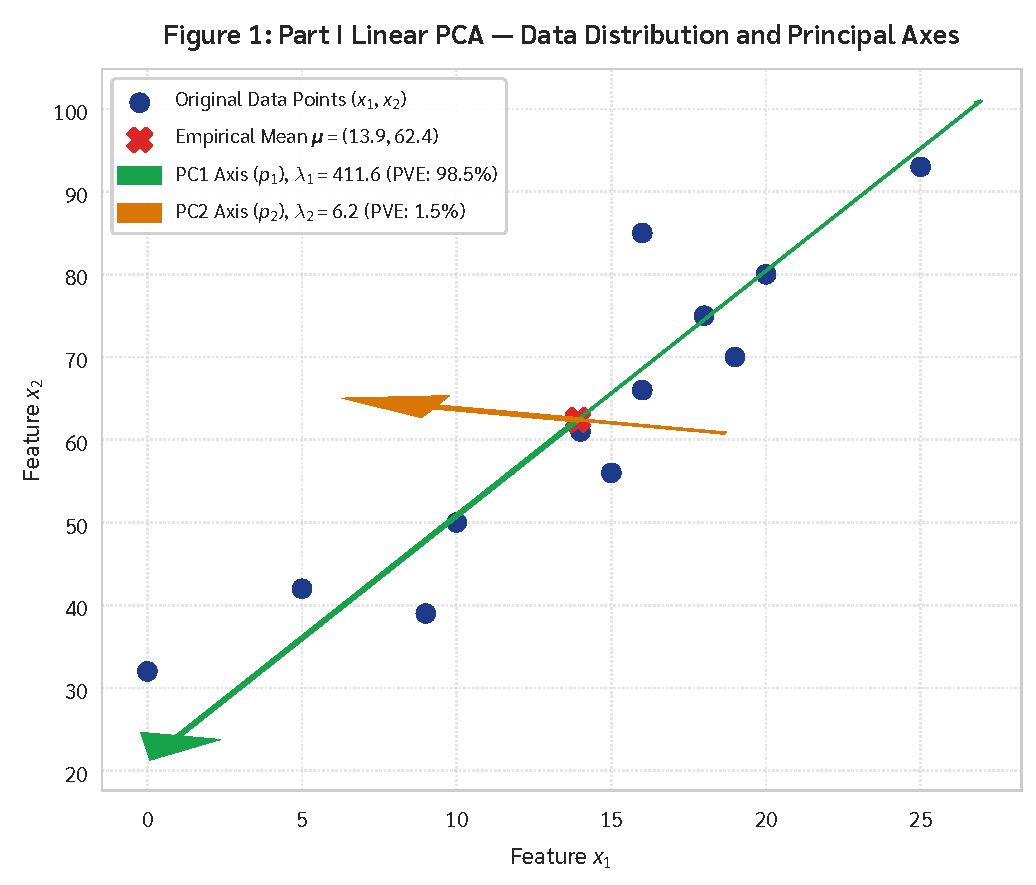
\includegraphics[width=\linewidth]{plot_1_linear_pca_geometry.pdf}
    \caption{การแจกแจงของข้อมูล 12 จุดและแกนองค์ประกอบหลัก $\mathbf{p}_1, \mathbf{p}_2$ ที่มีจุดกำเนิด ณ จุดเฉลี่ย $\boldsymbol{\mu}$}
    \label{fig:linear_pca_geom}
\end{minipage}\hfill
\begin{minipage}[t]{0.485\textwidth}
    \centering
    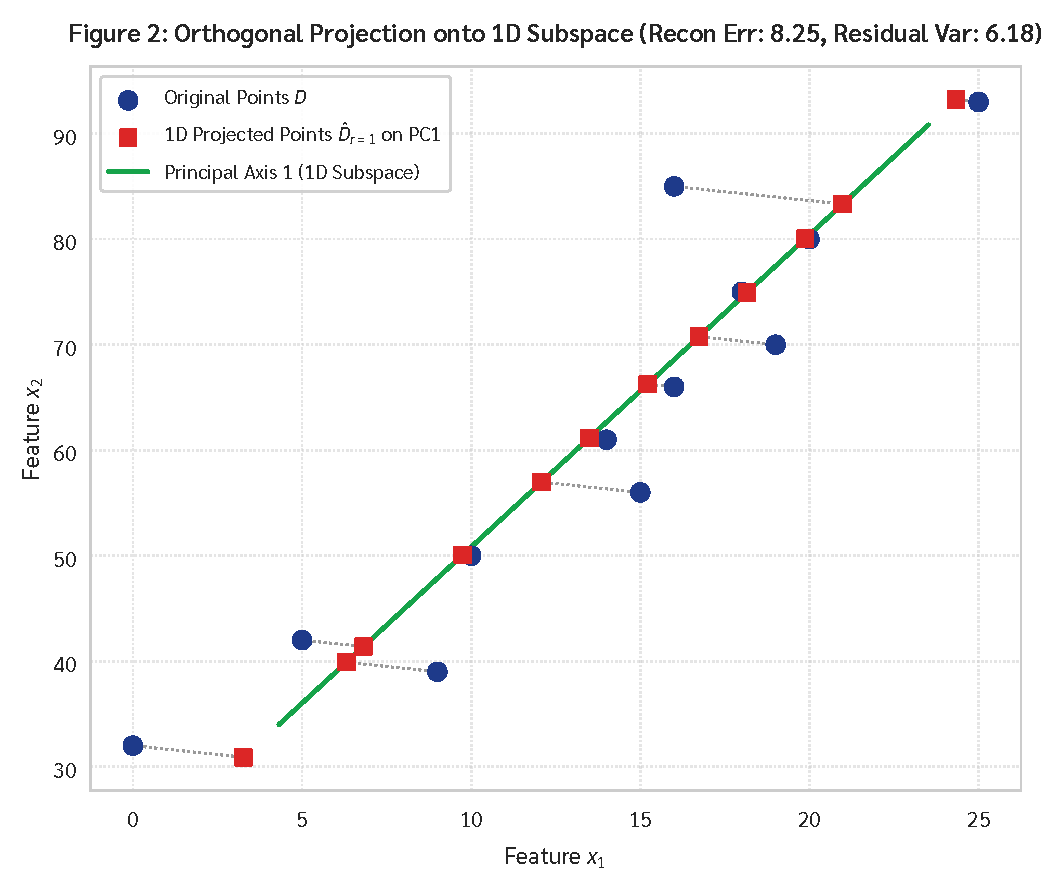
\includegraphics[width=\linewidth]{plot_2_projection_reconstruction.pdf}
    \caption{การฉายข้อมูลตั้งฉากลงบนปริภูมิย่อย 1 มิติ (PC1) และเส้นระยะตกค้าง (Residual Projection Lines)}
    \label{fig:proj_recon}
\end{minipage}
\end{figure}

\clearpage
% =========================================================================
% SECTION 3
% =========================================================================
\section*{3. คุณลักษณะและโครงสร้างของชุดข้อมูล MTCARS (Part II)\newline \large(Dataset Architecture \& Exploratory Analysis)}

ชุดข้อมูล \textbf{MTCARS} จากชีต \codevar{MTCARS} ในไฟล์ \codevar{dimensionality-reduction.xlsx} ประกอบด้วยข้อมูลรถยนต์จำนวน $32$ รุ่น และมีคุณลักษณะเชิงวิศวกรรม $11$ ตัวแปร ได้แก่:
\begin{table}[H]
\centering
\small
\begin{tabular}{lllcc}
\toprule
\textbf{ตัวแปร} & \textbf{ความหมายเชิงกายภาพ} & \textbf{หน่วยการวัด} & \textbf{Mean} & \textbf{Variance ($\sigma^2$)} \\
\midrule
\codevar{mpg}  & อัตราสิ้นเปลืองน้ำมัน & ไมล์ต่อแกลลอน & 20.09 & 36.32 \\
\codevar{cyl}  & จำนวนกระบอกสูบ & สูบ (4, 6, 8) & 6.19 & 3.19 \\
\codevar{disp} & ปริมาตรกระบอกสูบ (Displacement) & ลูกบาศก์นิ้ว (cu.in.) & 230.72 & \textbf{15,360.80} \\
\codevar{hp}   & แรงม้าสูงสุด (Gross Horsepower) & แรงม้า (hp) & 146.69 & \textbf{4,700.87} \\
\codevar{drat} & อัตราทดเฟืองท้าย & อัตราส่วน & 3.60 & 0.29 \\
\codevar{wt}   & น้ำหนักรถยนต์ & 1,000 ปอนด์ & 3.22 & 0.96 \\
\codevar{qsec} & เวลาเร่งความเร็วระยะ 1/4 ไมล์ & วินาที & 17.85 & 3.19 \\
\codevar{vs}   & การจัดวางกระบอกสูบ (0=V, 1=Straight) & ไบนารี & 0.44 & 0.25 \\
\codevar{am}   & ระบบเกียร์ (0=Auto, 1=Manual) & ไบนารี & 0.41 & 0.25 \\
\codevar{gear} & จำนวนเกียร์เดินหน้า & เกียร์ & 3.69 & 0.54 \\
\codevar{carb} & จำนวนคาร์บูเรเตอร์ & ตัว & 2.81 & 2.61 \\
\bottomrule
\end{tabular}
\caption{สถิติเชิงพรรณนาและสเกลความแปรปรวนของ 11 คุณลักษณะในชุดข้อมูล MTCARS}
\end{table}

ความแตกต่างอย่างมหาศาลของสเกลความแปรปรวนเห็นได้ชัดเจนในภาพ Figure 3: ตัวแปร \codevar{disp} ($\sigma^2 = 15,360.8$) และ \codevar{hp} ($\sigma^2 = 4,700.9$) มีขนาดใหญ่กว่า \codevar{wt}, \codevar{vs}, \codevar{am} กว่าหลายพันเท่า ซึ่งเป็นปัจจัยวิกฤตที่ส่งผลต่อพฤติกรรมของ PCA

\begin{figure}[H]
\centering
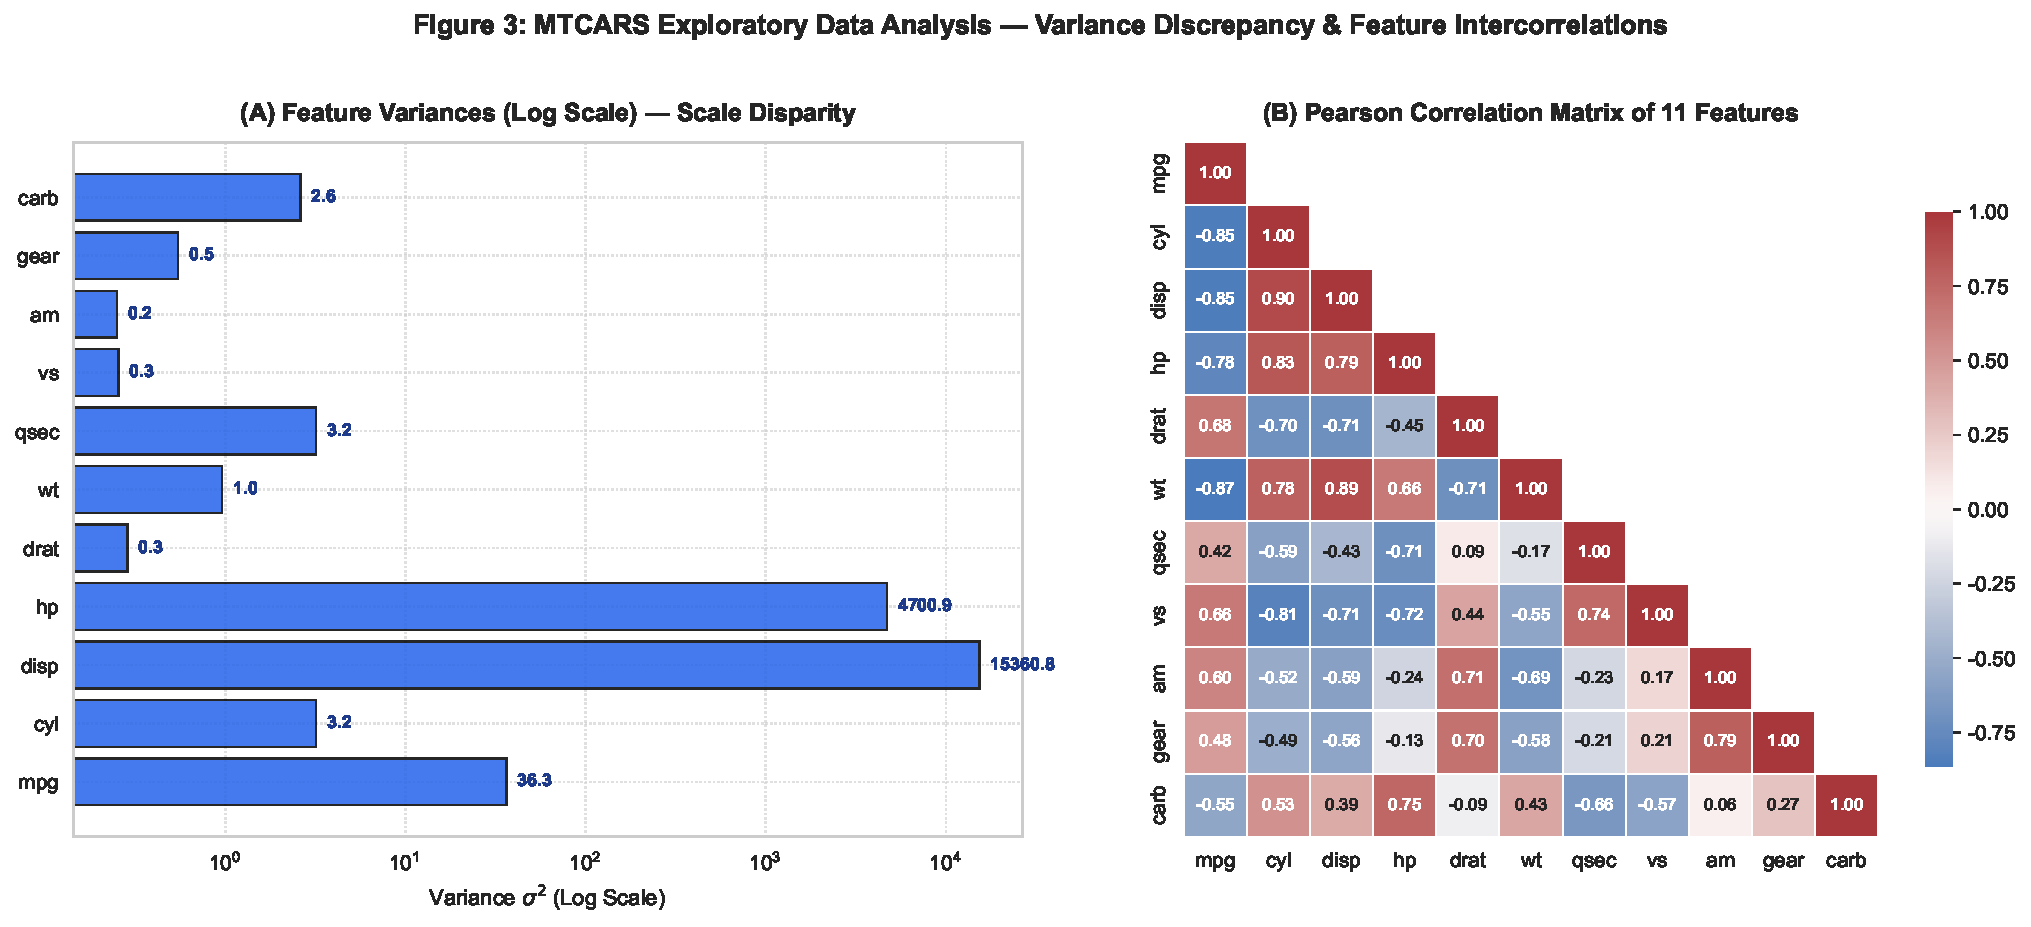
\includegraphics[width=0.86\linewidth]{plot_3_mtcars_eda_corrmat.pdf}
\caption{การกระจายตัวของความแปรปรวน (Log Scale) และเมทริกซ์สหสัมพันธ์เพียร์สันของ MTCARS}
\end{figure}

\clearpage
% =========================================================================
% SECTION 4
% =========================================================================
\section*{4. การเปรียบเทียบเชิงวิเคราะห์ระหว่าง Unstandardized และ Standardized PCA\newline \large(Comparative Analysis: Unstandardized vs. Standardized PCA)}

เมื่อทำการคำนวณ PCA บนข้อมูลดิบที่ไม่ผ่านการปรับมาตรฐาน เปรียบเทียบกับข้อมูลที่ผ่านการปรับมาตรฐานด้วย \codevar{StandardScaler()} ผลลัพธ์ที่ได้มีความแตกต่างกันอย่างมีนัยสำคัญอย่างยิ่ง:

\begin{table}[H]
\centering
\small
\begin{tabular}{lrrrrrr}
\toprule
& \multicolumn{3}{c}{\textbf{Unstandardized PCA}} & \multicolumn{3}{c}{\textbf{Standardized PCA}} \\
\cmidrule(lr){2-4} \cmidrule(lr){5-7}
\textbf{PC} & \textbf{Eigenvalue} & \textbf{PVE (\%)} & \textbf{Cum. PVE (\%)} & \textbf{Eigenvalue} & \textbf{PVE (\%)} & \textbf{Cum. PVE (\%)} \\
\midrule
PC1 & 18,946.06 & \textbf{92.70\%} & 92.70\% & 6.8216 & \textbf{60.08\%} & 60.08\% \\
PC2 & 1,479.25  & 7.24\%  & \textbf{99.94\%} & 2.7360 & 24.10\% & 84.17\% \\
PC3 & 10.74     & 0.05\%  & 99.98\% & 0.6474 & 5.70\%  & \textbf{89.87\%} \\
PC4 & 2.65      & 0.01\%  & 99.99\% & 0.2783 & 2.45\%  & \textbf{92.32\%} \\
PC5 & 1.09      & 0.01\%  & 100.00\% & 0.2307 & 2.03\%  & 94.36\% \\
PC6 & 0.32      & 0.00\%  & 100.00\% & 0.2178 & 1.92\%  & 96.28\% \\
PC7 & 0.17      & 0.00\%  & 100.00\% & 0.1394 & 1.23\%  & 97.51\% \\
PC8 & 0.08      & 0.00\%  & 100.00\% & 0.1276 & 1.12\%  & 98.63\% \\
PC9 & 0.03      & 0.00\%  & 100.00\% & 0.0792 & 0.70\%  & 99.33\% \\
PC10& 0.01      & 0.00\%  & 100.00\% & 0.0538 & 0.47\%  & 99.80\% \\
PC11& 0.00      & 0.00\%  & 100.00\% & 0.0230 & 0.20\%  & 100.00\% \\
\midrule
\textbf{Total} & \textbf{20,440.40} & \textbf{100.00\%} & — & \textbf{11.3548} & \textbf{100.00\%} & — \\
\bottomrule
\end{tabular}
\caption{ตารางเปรียบเทียบสเปกตรัมของค่าลักษณะเฉพาะ สัดส่วน PVE และความแปรปรวนสะสม}
\end{table}

\begin{figure}[H]
\centering
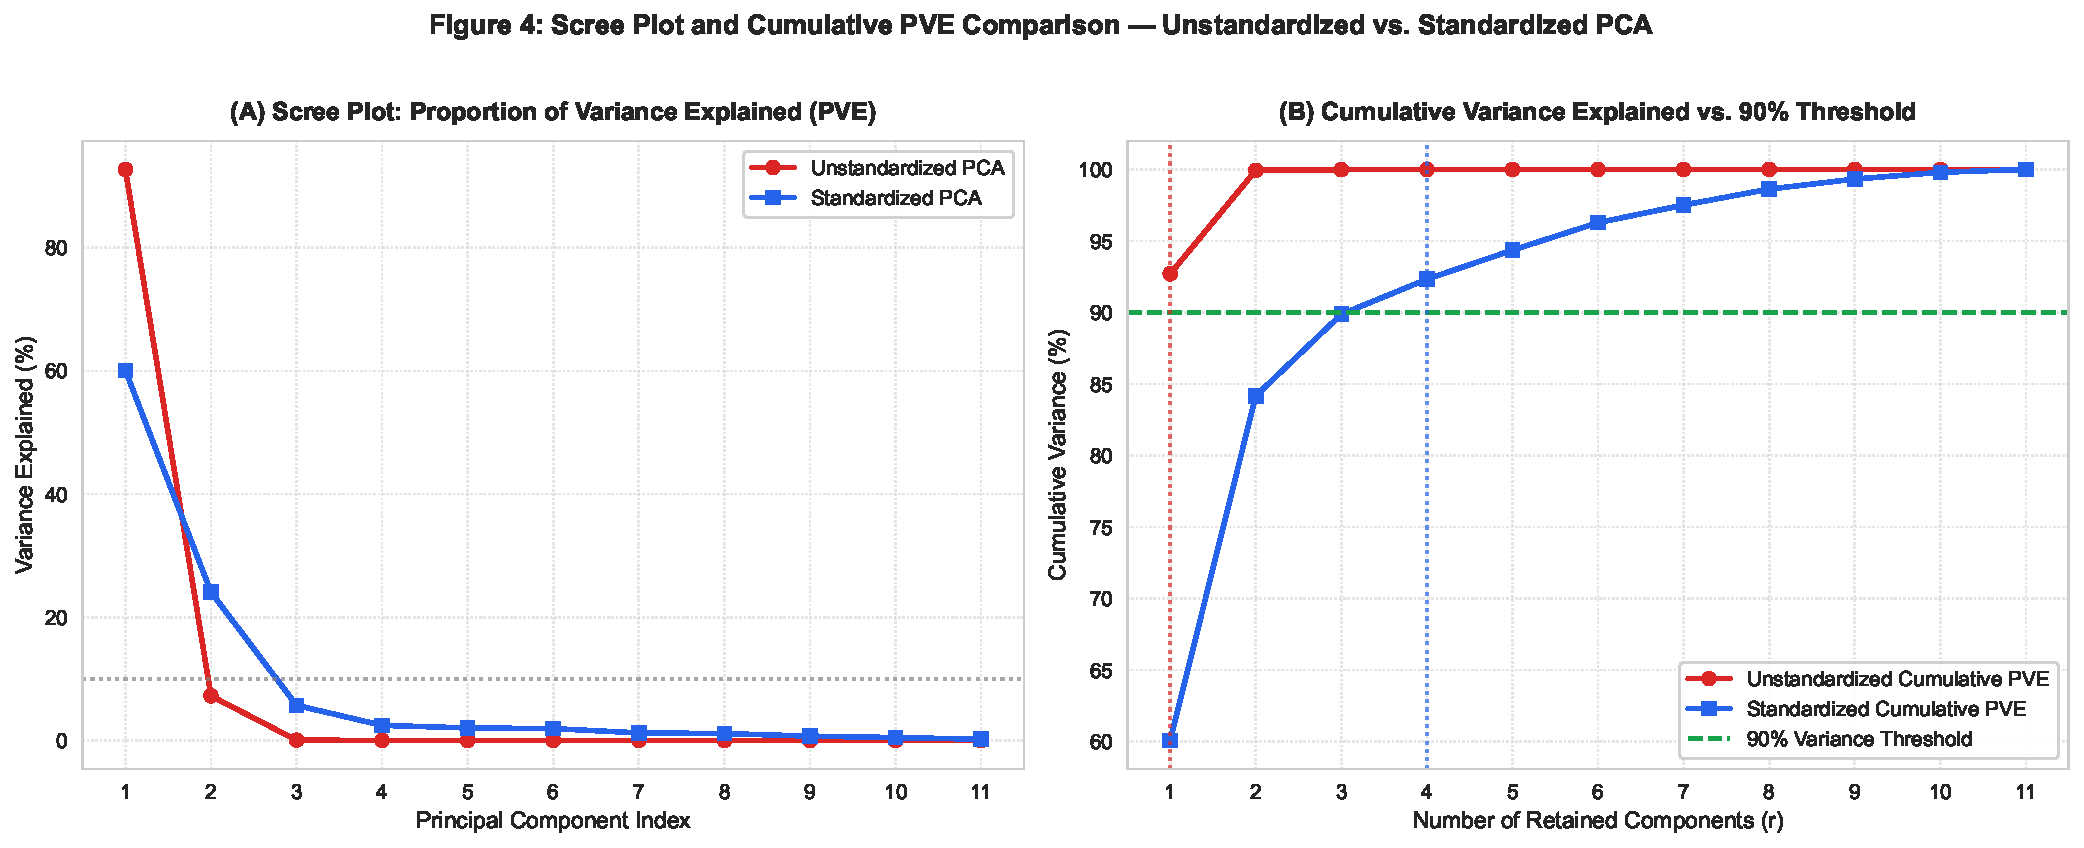
\includegraphics[width=0.86\linewidth]{plot_4_scree_pve_comparison.pdf}
\caption{การเปรียบเทียบ Scree Plot และความแปรปรวนสะสมระหว่างสองระเบียบวิธี}
\end{figure}

จากตารางและแผนภาพ Scree Plot (Figure 4) แสดงให้เห็นอย่างเด่นชัดว่า ใน Unstandardized PCA เส้นกราฟ PVE ทอดดิ่งลงแทบเป็นศูนย์ทันทีหลัง PC1 ($\text{PVE}_1 = 92.70\%$) ขณะที่ Standardized PCA เส้น PVE มีการกระจายตัวอย่างราบรื่น โดยต้องสะสมถึง PC4 จึงจะก้าวข้ามเกณฑ์ $90\%$ ($\text{Cum. PVE}_4 = 92.32\%$)

\clearpage
\subsection*{4.1 การเปรียบเทียบการกระจายค่าน้ำหนักตัวแปรในแกนองค์ประกอบหลักที่ 1\newline \normalsize(PC1 Loadings Distribution \& Feature Scale Shift Analysis)}

\begin{figure}[H]
\centering
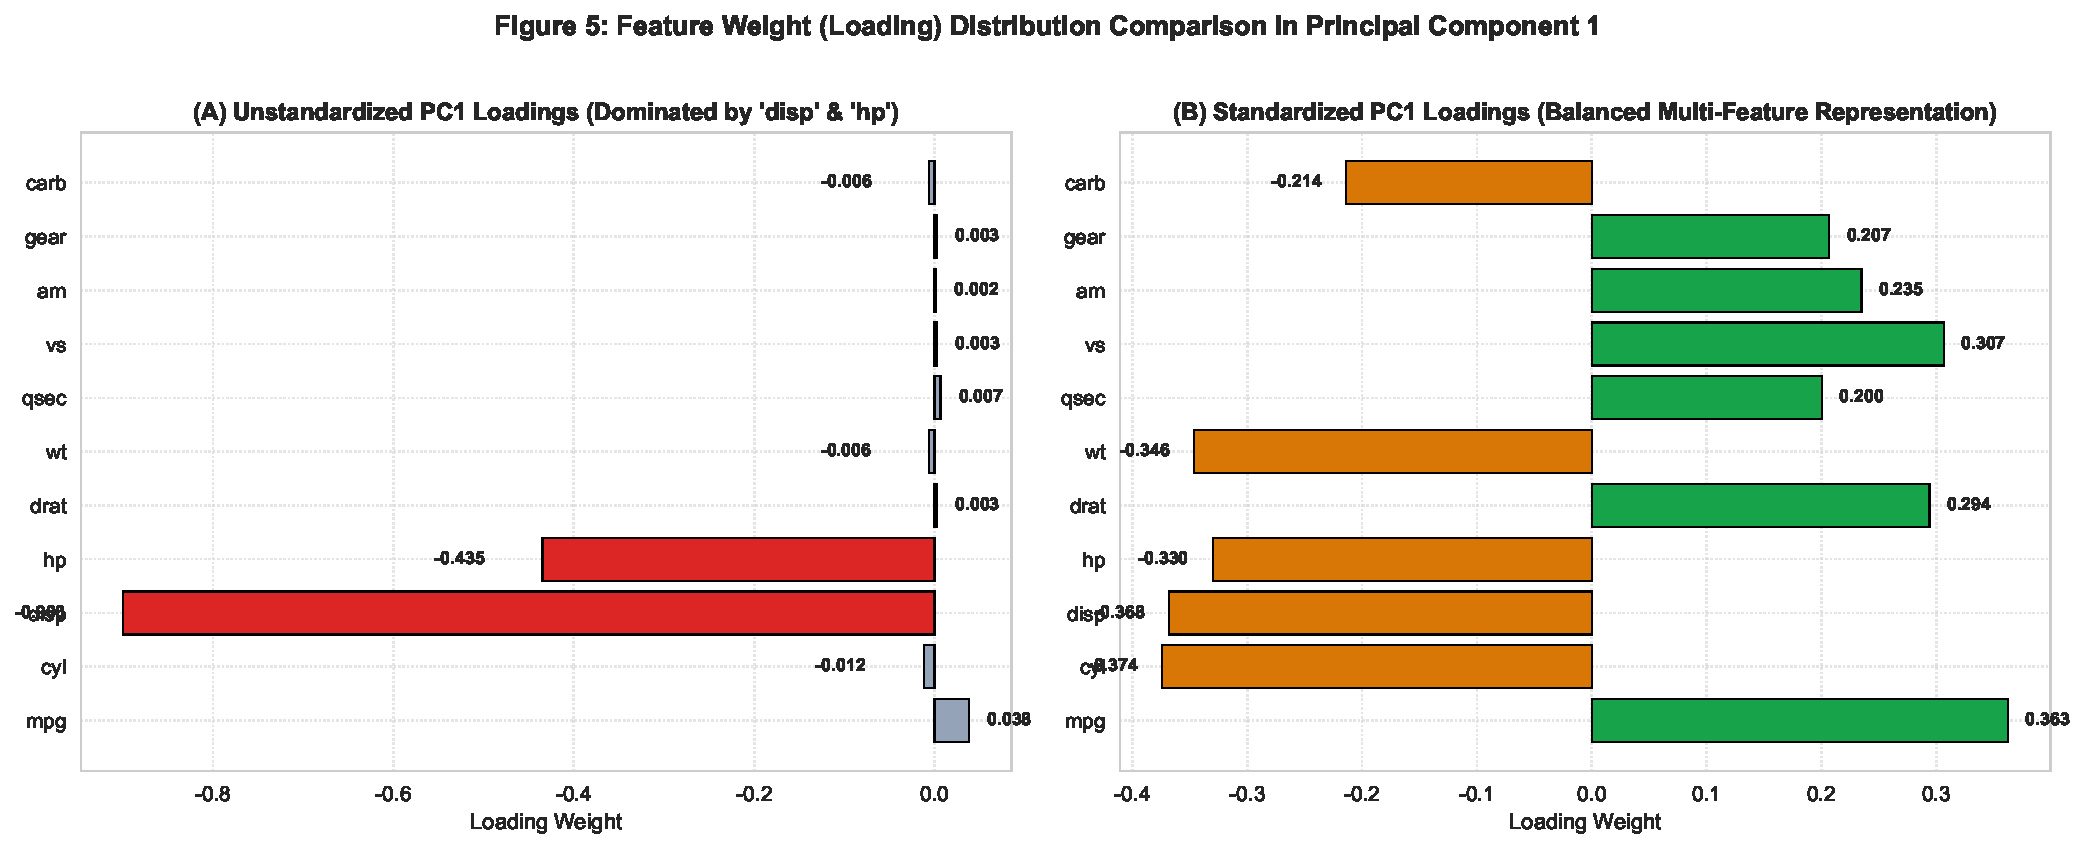
\includegraphics[width=0.86\linewidth]{plot_5_pc_loadings_barplot.pdf}
\caption{การเปรียบเทียบค่าน้ำหนักตัวแปร (Loadings) ในแกน PC1}
\end{figure}

จากแผนภูมิแท่งเปรียบเทียบ (Figure 5) ชี้ให้เห็นปรากฏการณ์สำคัญเชิงทฤษฎี:
\begin{enumerate}[leftmargin=1.5em, itemsep=2pt, topsep=2pt]
    \item \textbf{การผูกขาดของสองตัวแปรใน Unstandardized PC1:} แกน PC1 ก่อนการปรับมาตรฐานประกอบด้วยค่าน้ำหนักของ \codevar{disp} ($-0.8996$) และ \codevar{hp} ($-0.4348$) คิดเป็นพลังงานเวกเตอร์รวม $0.8996^2 + 0.4348^2 = 0.9983$ หรือ $99.83\%$ ของความยาวเวกเตอร์หนึ่งหน่วย ส่งผลให้ตัวแปรสำคัญอีก 9 ตัวแทบไม่มีผลต่อคะแนน PC1 เลย
    \item \textbf{การกระจายตัวอย่างสมดุลใน Standardized PC1:} ภายหลังการปรับมาตรฐาน ตัวแปรทุกตัวมีสเกลความแปรปรวนเริ่มต้นเท่ากันที่ $1.0$ ค่าน้ำหนักจึงถูกจัดสรรอย่างยุติธรรม โดยตัวแปร \codevar{cyl} ($-0.3739$), \codevar{disp} ($-0.3682$), \codevar{mpg} ($+0.3625$), \codevar{wt} ($-0.3461$), \codevar{hp} ($-0.3301$) และ \codevar{vs} ($+0.3065$) ล้วนมีค่าน้ำหนักอยู่ในช่วง $|w_j| \in [0.30, 0.38]$ ซึ่งสะท้อนถึงการสังเคราะห์ความสัมพันธ์พหุคูณ (Multivariate Intercorrelations) ของยานยนต์ที่แท้จริง
\end{enumerate}

% =========================================================================
% SECTION 5: QUESTIONS AND ANSWERS (EXACTLY 1 PAGE PER QUESTION)
% =========================================================================
\clearpage
\section*{5. การตอบคำถามประจำการทดลองและการวินิจฉัยเชิงวิศวกรรม\newline \large(Experiment Question Solutions \& Engineering Insights)}
\vspace{-0.6em}
\subsection*{คำถามที่ 2.1: การวิเคราะห์ PCA บนข้อมูลไม่ปรับมาตรฐาน\newline \normalsize(Question 2.1: PCA on Unstandardized Dataset)}
\vspace{-0.5em}

\begin{ansbox}[fontupper=\small, left=6pt, right=6pt, top=3pt, bottom=3pt]
\textbf{โจทย์ (Question 2.1 Prompt)}:
\begin{itemize}[leftmargin=1.2em, itemsep=0pt, topsep=0pt, parsep=0pt]
    \item[(a)] \textit{How many PCs are sufficient to explain at least approximately 90\% of the total variation in the data?}
    \item[(b)] \textit{Which of the original features get large weights (loadings) in PC1?}
\end{itemize}

\vspace{-0.2em}
\noindent\rule{\linewidth}{0.4pt}
\vspace{-0.2em}

\noindent\textbf{\normalsize (a) จำนวน PCs ที่เพียงพอสำหรับอธิบายความแปรปรวนรวม $\ge 90\%$}\par\vspace{0.05em}
\textbf{คำตอบ (ANSWER):} ใช้เพียง \textbf{1 PC (PC1 เพียงแกนเดียว)} ก็เพียงพออย่างสมบูรณ์\\[0.05em]
\textbf{หลักฐานเชิงประจักษ์และการพิสูจน์เชิงคณิตศาสตร์ (Empirical Proof):}
\begin{itemize}[leftmargin=1.3em, itemsep=0.5pt, topsep=0.5pt]
    \item ความแปรปรวนรวมทั้งหมด: $\text{Total Variance} = \text{tr}(\boldsymbol{\Sigma}_{\text{unstd}}) = \sum_{j=1}^{11} \lambda_j = 20,440.4042$
    \item ค่าลักษณะเฉพาะสูงสุดอันดับแรกมีค่าสูงถึง $\lambda_1 = 18,946.0620$
    \item สัดส่วนความแปรปรวนที่อธิบายได้โดย $\text{PC1}$: $\text{PVE}_1 = \frac{\lambda_1}{\sum_{k=1}^{11} \lambda_k} = \frac{18,946.0620}{20,440.4042} = \mathbf{92.6893\% \approx 92.70\%}$
    \item ค่า $\text{PVE}_1 = 92.70\% > 90\%$ ทำให้การคงไว้เพียง $r=1$ มิติ ครอบคลุมสารสนเทศเกินเกณฑ์ทันที และหากใช้ $r=2$ ($\text{PC1} + \text{PC2}$) จะอธิบายได้สูงถึง $\mathbf{99.94\%}$
\end{itemize}

\vspace{-0.1em}
\noindent\textbf{\normalsize (b) ตัวแปรตั้งต้นที่ได้รับค่าน้ำหนัก (Loadings) สูงในแกน PC1}\par\vspace{0.05em}
\textbf{คำตอบ (ANSWER):} ตัวแปรที่ได้รับค่าน้ำหนักสูงอย่างมีนัยสำคัญคือ \textbf{\codevar{disp} (Displacement)} และ \textbf{\codevar{hp} (Horsepower)}\\[0.05em]
\textbf{ตารางแจกแจงค่าน้ำหนักของเวกเตอร์ $\mathbf{p}_1$ ใน Unstandardized PCA:}
\vspace{-0.2em}

\noindent\centering
\resizebox{\linewidth}{!}{
\begin{tabular}{lrrrrrrrrrrr}
\toprule
\textbf{Feature} & \codevar{disp} & \codevar{hp} & \codevar{mpg} & \codevar{cyl} & \codevar{qsec} & \codevar{wt} & \codevar{carb} & \codevar{drat} & \codevar{vs} & \codevar{gear} & \codevar{am} \\
\midrule
\textbf{Loading} & \textbf{-0.8996} & \textbf{-0.4348} & 0.0381 & -0.0120 & 0.0067 & -0.0062 & -0.0058 & 0.0027 & 0.0027 & 0.0026 & 0.0020 \\
\textbf{Abs (\%)} & \textbf{89.96\%} & \textbf{43.48\%} & 3.81\% & 1.20\% & 0.67\% & 0.62\% & 0.58\% & 0.27\% & 0.27\% & 0.26\% & 0.20\% \\
\bottomrule
\end{tabular}
}
\par\vspace{0.2em}
\raggedright
\textbf{คำอธิบายเหตุผลทางกายภาพและคณิตศาสตร์ (Root Cause Analysis):}
\begin{enumerate}[leftmargin=1.3em, itemsep=0.5pt, topsep=0.5pt]
    \item \textbf{การครอบงำของสเกลหน่วยวัด (Scale Domination):} ตัวแปร \codevar{disp} มีความแปรปรวน $\sigma^2 = 15,360.80$ คิดเป็น \textbf{75.15\%} ของความแปรปรวนทั้งระบบ และ \codevar{hp} มีความแปรปรวน $\sigma^2 = 4,700.87$ คิดเป็น \textbf{23.00\%} รวมสองตัวแปรครองความแปรปรวนไปถึง \textbf{98.15\%}
    \item \textbf{การละเลยตัวแปรสเกลเล็ก:} ตัวแปรสำคัญอย่าง \codevar{wt} ($\sigma^2 = 0.96$), \codevar{am} ($\sigma^2 = 0.25$) หรือ \codevar{drat} ($\sigma^2 = 0.29$) มีความแปรปรวนต่ำกว่าหลักพันเท่า สมการจึงเลือกลำดับเวกเตอร์ที่ขนานกับแกน \codevar{disp} แทบทั้งหมด โดยที่ตัวแปรอื่นทั้ง 9 ตัวมีน้ำหนักใกล้ศูนย์ ($|w| \le 0.038$)
    \item \textbf{ข้อสรุปทางระเบียบวิธี:} ใน Unstandardized PCA แกน $\text{PC1}$ ไม่ได้สะท้อนความสัมพันธ์พหุคูณของรถยนต์ แต่ทำหน้าที่เป็นเพียง ``ตัวแทนของตัวแปร \codevar{disp}'' เท่านั้น
\end{enumerate}
\end{ansbox}

% =========================================================================
% QUESTION 2.2 PAGE (EXACTLY 1 FULL PAGE)
% =========================================================================
\clearpage
\subsection*{คำถามที่ 2.2: การวิเคราะห์ PCA แบบปรับมาตรฐานและเปรียบเทียบเชิงลึก\newline \normalsize(Question 2.2: PCA on Standardized Dataset \& Comparative Rationale)}
\vspace{-0.5em}

\begin{ansbox}[fontupper=\small, left=6pt, right=6pt, top=3pt, bottom=3pt]
\textbf{โจทย์ (Question 2.2 Prompt)}:
\begin{itemize}[leftmargin=1.2em, itemsep=0pt, topsep=0pt, parsep=0pt]
    \item[(a)] \textit{How many PCs are sufficient to explain at least approximately 90\% of the total variation in the data?}
    \item[(b)] \textit{Which of the original features get large weights (loadings) in PC1?}
    \item[(c)] \textit{Do the PCA outputs differ significantly between standardizing and not standardizing the dataset before applying PCA? Explain the results.}
\end{itemize}

\vspace{-0.2em}
\noindent\rule{\linewidth}{0.4pt}
\vspace{-0.2em}

\noindent\textbf{\normalsize (a) จำนวน PCs ที่เพียงพอสำหรับอธิบายความแปรปรวนรวม $\ge 90\%$}\par\vspace{0.05em}
\textbf{คำตอบ (ANSWER):} ต้องใช้ \textbf{4 PCs} เพื่อให้ครอบคลุมเกิน $90\%$ อย่างสมบูรณ์ ($\mathbf{92.32\%}$) หรืออนุโลมให้เป็น \textbf{3 PCs} หากยอมรับค่าประมาณใกล้เคียง ($\mathbf{89.87\% \approx 90\%}$)
\begin{itemize}[leftmargin=1.3em, itemsep=0.5pt, topsep=0.5pt]
    \item ความแปรปรวนสะสมใน Standardized PCA: $\text{PC1} = 60.08\%$, $\text{PC1-2} = 84.17\%$, $\text{PC1-3} = 89.87\%$, $\text{PC1-4} = \mathbf{92.32\%}$
    \item เมื่อปรับมาตรฐานให้ทุกตัวแปรมีความแปรปรวนเท่ากันที่ $\sigma^2 = 1.0$ สารสนเทศจะไม่กระจุกตัวที่ตัวแปรเดี่ยว จึงต้องสะสมถึง 4 แกนเพื่อรวบรวมข้อมูลให้ครบตามเกณฑ์
\end{itemize}

\vspace{-0.1em}
\noindent\textbf{\normalsize (b) ตัวแปรตั้งต้นที่ได้รับค่าน้ำหนัก (Loadings) สูงในแกน PC1}\par\vspace{0.05em}
\textbf{คำตอบ (ANSWER):} ใน Standardized PCA \textbf{ทุกตัวแปรมีบทบาทร่วมกันอย่างสมดุล} ($|w_j| \in [0.20, 0.37]$) โดยแบ่งขั้วการกระจายตัวออกเป็น 2 กลุ่มตรงข้ามอย่างชัดเจน:
\begin{enumerate}[leftmargin=1.3em, itemsep=0.5pt, topsep=0.5pt]
    \item \textbf{กลุ่มค่าน้ำหนักลบ (Power, Size \& Weight Axis):} \codevar{cyl} ($-0.3739$), \codevar{disp} ($-0.3682$), \codevar{wt} ($-0.3461$), \codevar{hp} ($-0.3301$), \codevar{carb} ($-0.2140$)
    \item \textbf{กลุ่มค่าน้ำหนักบวก (Fuel Efficiency \& Transmission Axis):} \codevar{mpg} ($+0.3625$), \codevar{vs} ($+0.3065$), \codevar{drat} ($+0.2942$), \codevar{am} ($+0.2349$), \codevar{gear} ($+0.2069$), \codevar{qsec} ($+0.2005$)
\end{enumerate}
\textbf{การตีความเชิงกายภาพ:} แกน $\text{PC1}$ แสดงถึงดัชนีวัดความประหยัดและความคล่องตัว ปะทะกับ ขนาดเครื่องยนต์ น้ำหนัก และกำลังขับเคลื่อน ซึ่งเป็น Trade-off หลักของวิศวกรรมยานยนต์

\vspace{-0.1em}
\noindent\textbf{\normalsize (c) การวิเคราะห์เปรียบเทียบว่าทำไมผลลัพธ์จึงแตกต่างกันอย่างมีนัยสำคัญยิ่ง}\par\vspace{0.05em}
\textbf{คำตอบ (ANSWER):} แตกต่างกันอย่างมหาศาลและมีความสำคัญเชิงรากฐานทางสถิติ (Dramatically Different) ด้วยเหตุผล 3 ประการ:
\begin{enumerate}[leftmargin=1.3em, itemsep=0.5pt, topsep=0.5pt]
    \item \textbf{ความหมายของเมทริกซ์ที่นำมาคำนวณ (Covariance vs Correlation Matrix):} Unstandardized PCA คำนวณบน Covariance Matrix ($\boldsymbol{\Sigma}$) ซึ่งขึ้นกับหน่วยวัด ขณะที่ Standardized PCA ปรับ $z = (x - \mu)/\sigma$ ทำให้คำนวณบน \textbf{Pearson Correlation Matrix ($\mathbf{R}$)} ซึ่งคงที่ต่อสเกล (Scale-Invariant)
    \item \textbf{การบิดเบือนทางเรขาคณิต (Geometric Distortion):} ใน Unstandardized PCA แกนข้อมูลถูกยืดออกตามหน่วยลูกบาศก์นิ้วของ \codevar{disp} ทำให้ทรงรีของข้อมูลชี้ไปในแนวแกน \codevar{disp} ตัวเดียว ขณะที่ Standardized PCA ปรับให้ความยาวข้อมูลทุกมิติมีสเกลเท่ากัน ทรงรีจึงหมุนตามสหสัมพันธ์ที่แท้จริง
    \item \textbf{ข้อเสนอแนะเชิงวิศวกรรม (Engineering Recommendation):} เมื่อคุณลักษณะมีหน่วยการวัดคนละประเภท \textbf{จำเป็นอย่างยิ่งที่จะต้องทำ Data Standardization ก่อนประยุกต์ใช้ PCA เสมอ} มิฉะนั้นผลลัพธ์จะถูกบิดเบือน
\end{enumerate}
\end{ansbox}

% =========================================================================
% SECTION 6
% =========================================================================
\clearpage
\section*{6. การตีความทางเรขาคณิตและการวิเคราะห์ 2D Biplot\newline \large(Geometric Interpretation \& 2D Biplot Semantic Diagnostics)}

เพื่อทำความเข้าใจเชิงลึกเกี่ยวกับการจัดกลุ่มและการกระจายตัวของรถยนต์ทั้ง 32 รุ่น เราสร้างแผนภาพ \textbf{2D PCA Biplot} โดยฉายจุดพิกัดของรถยนต์ลงบนระนาบ $(\text{PC1}, \text{PC2})$ ควบคู่กับเวกเตอร์ค่าน้ำหนักของตัวแปรทั้ง 11 ตัว (Figure 6)

\begin{figure}[H]
\centering
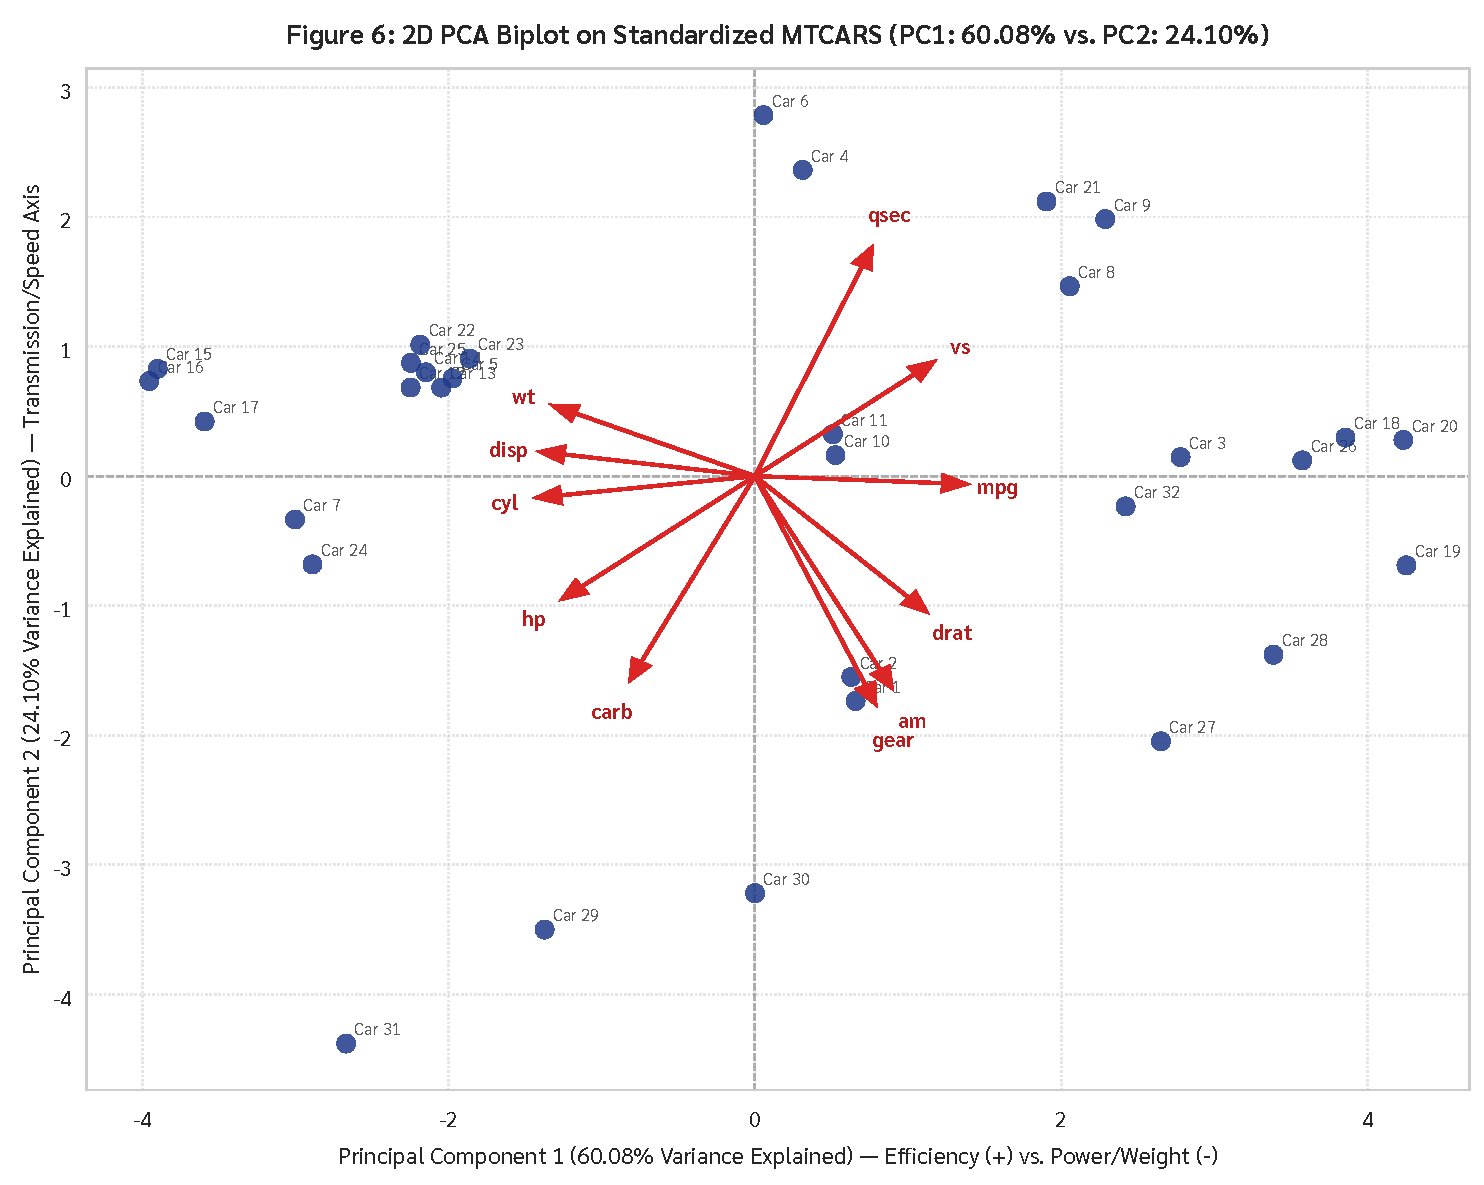
\includegraphics[width=0.68\linewidth]{plot_6_pca_biplot_2d.pdf}
\caption{แผนภาพ 2D PCA Biplot บนชุดข้อมูล MTCARS ที่ผ่านการปรับมาตรฐาน (Standardized)}
\end{figure}

\subsection*{6.1 การวิเคราะห์กลุ่มยานยนต์เชิงความหมาย\\ \normalsize(Semantic Vehicle Clustering via 2D Biplot)}
จากแผนภาพ Figure 6 สามารถจำแนกประชากรรถยนต์ออกเป็น 3 กลุ่มพฤติกรรมหลักอย่างชัดเจน:
\begin{enumerate}[leftmargin=1.5em, itemsep=1.5pt, topsep=1.5pt]
    \item \textbf{กลุ่มรถยนต์สมรรถนะสูงและตัวถังขนาดใหญ่ (Muscle \& Luxury Heavyweights):}
    กระจุกตัวอยู่ในควอแดรนต์ซ้าย (ค่า $\text{PC1} < -2.0$) เช่น \textit{Lincoln Continental, Cadillac Fleetwood, Chrysler Imperial, Camaro Z28} รถยนต์กลุ่มนี้มีเวกเตอร์ชี้ไปในทิศทางเดียวกับ \codevar{disp}, \codevar{cyl}, \codevar{wt}, \codevar{hp} สะท้อนถึงเครื่องยนต์ V8 ขนาดใหญ่ กินน้ำมันสูง และมีน้ำหนักตัวถังมาก
    \item \textbf{กลุ่มรถยนต์ประหยัดพลังงานและขนาดกะทัดรัด (Economy Compacts):}
    กระจุกตัวอยู่ในควอแดรนต์ขวาบน (ค่า $\text{PC1} > +2.0, \text{PC2} > 0$) เช่น \textit{Toyota Corolla, Fiat 128, Honda Civic, Lotus Europa} อยู่ในทิศทางเดียวกับเวกเตอร์ \codevar{mpg}, \codevar{qsec}, \codevar{vs} แสดงถึงเครื่องยนต์ 4 สูบแถวเรียง ประหยัดน้ำมัน และน้ำหนักเบา
    \item \textbf{กลุ่มรถสปอร์ตเกียร์ธรรมดาความเร็วสูง (Agile Manual Sports Cars):}
    กระจุกตัวอยู่ในควอแดรนต์ขวาล่าง เช่น \textit{Porsche 914-2, Ferrari Dino, Ford Pantera L} สอดคล้องกับทิศทางของเวกเตอร์ \codevar{am}, \codevar{gear}, \codevar{drat} ซึ่งเน้นอัตราทดเกียร์ธรรมดาและความคล่องตัวสูง
\end{enumerate}

\clearpage
\subsection*{6.2 การตรวจสอบข้อผิดพลาดในการฟื้นฟูข้อมูล\\ \normalsize(Reconstruction Error Curve Analysis)}
Figure 7 แสดงกราฟข้อผิดพลาดสัมพัทธ์ในการฟื้นฟูข้อมูล $\frac{\|\mathbf{X} - \hat{\mathbf{X}}_r\|_F}{\|\mathbf{X}\|_F} \times 100\%$ เมื่อเพิ่มจำนวนมิติ $r$ จาก 1 ถึง 11 จะเห็นว่าค่าความผิดพลาดลดลงสู่ $0.00\%$ เมื่อ $r=11$ ยืนยันคุณสมบัติการแปลงย้อนกลับแบบไม่สูญเสียสารสนเทศ (Lossless Reconstruction) ตามทฤษฎี Spectral Theorem

\begin{figure}[H]
\centering
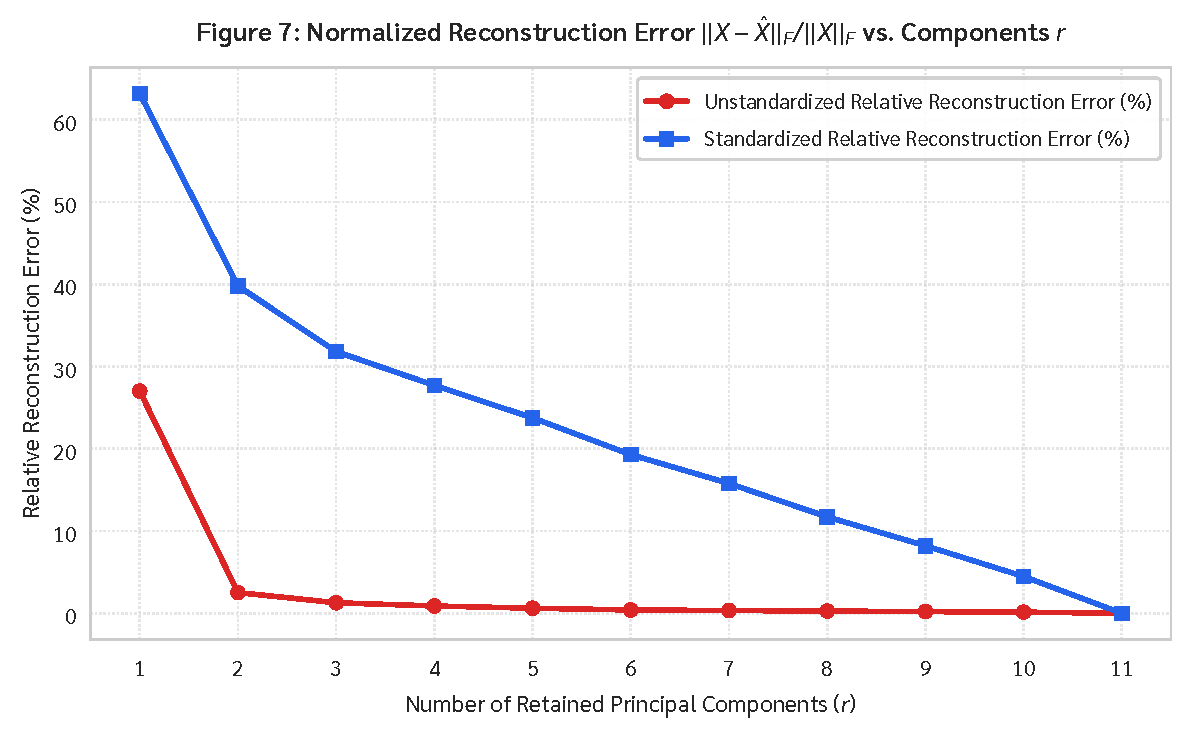
\includegraphics[width=0.55\linewidth]{plot_7_reconstruction_error.pdf}
\caption{กราฟ Normalized Reconstruction Error เทียบกับจำนวนองค์ประกอบหลักที่คงไว้ ($r$)}
\end{figure}

% =========================================================================
% SECTION 7
% =========================================================================
\section*{7. สรุปผลการทดลองและแนวปฏิบัติที่ดีที่สุดในงานวิศวกรรมข้อมูล\newline \large(Conclusions \& Practical Recommendations)}

การทดลองใน Assignment 7 นี้ให้ข้อสรุปเชิงทฤษฎีและการประยุกต์ใช้ที่สำคัญยิ่ง 3 ประการ:
\begin{enumerate}[leftmargin=1.5em, itemsep=1.5pt, topsep=1.5pt]
    \item \textbf{ความสำคัญสูงสุดของการปรับมาตรฐานข้อมูล (Standardization is Mandatory):} การทำ PCA บนข้อมูลที่ยังไม่ได้ปรับมาตรฐานจะทำให้ตัวแปรที่มีหน่วยวัดสเกลใหญ่ครอบงำระบบโดยสิ้นเชิง การปรับมาตรฐานให้มี $\mu=0, \sigma^2=1$ จะแปลงปัญหาเป็นการแยกตัวประกอบเฉพาะบน Correlation Matrix ซึ่งรักษาความสัมพันธ์ที่แท้จริงของระบบ
    \item \textbf{เกณฑ์การเลือกจำนวนมิติที่เหมาะสม ($r$ Selection Criteria):} ในการลดมิติข้อมูล ควรพิจารณาร่วมกันระหว่างเกณฑ์ความแปรปรวนสะสม ($\ge 90\%$), จุดหักศอกบน Scree Plot (Elbow Method), และค่าลักษณะเฉพาะที่มากกว่า $1.0$ (Kaiser Criterion) ซึ่งสำหรับ MTCARS การเลือก $r=4$ มิติสามารถลดมิติข้อมูลลงได้ถึง $63.6\%$ ขณะที่รักษาความแปรปรวนไว้ได้สูงถึง $92.32\%$
    \item \textbf{บทบาทของ Biplot ในการวิเคราะห์เชิงสำรวจ:} 2D Biplot เป็นเครื่องมือทัศนวิเคราะห์ (Visual Analytics) ที่ทรงพลังในการทำความเข้าใจโครงสร้างประชากรข้อมูล การจัดกลุ่มธรรมชาติ และทิศทางของปัจจัยขับเคลื่อนพร้อมกันในแผนภาพเดียว
\end{enumerate}

% =========================================================================
% APPENDIX: FULL JUPYTER NOTEBOOK CODE & OUTPUT
% =========================================================================
\clearpage
\appendix
\raggedbottom
\section*{Appendix: Full Jupyter Notebook Code \& Output}

รายละเอียดต่อไปนี้คือโค้ด Python ที่ใช้แก้ปัญหาและวิเคราะห์แบบจำลอง Dimensionality Reduction via PCA บนชุดข้อมูล MTCARS พร้อมผลลัพธ์และกราฟทั้งหมด ซึ่งได้รันจริงจาก Jupyter Notebook (\texttt{[Lab] Dimensionality Reduction.ipynb} หรือ \texttt{67\_1003\_1027\_1042\_1045\_1067.ipynb})

\begin{tcolorbox}[colback=blue!5!white,colframe=blue!75!black,halign=left,before upper={\sloppy\raggedright},title=\textbf{Jupyter Notebook: [Lab] Dimensionality Reduction.ipynb\\ (ไฟล์ส่งงานหลัก: 67\_1027\_1042.ipynb)}]
โค้ด ผลลัพธ์ และการพล็อตภาพทั้งหมดด้านล่างเป็นการรันจริงจาก Jupyter Notebook
\end{tcolorbox}

\vspace{0.6em}
\needspace{3\baselineskip}
\noindent\textbf{\small [In 1]:}
\begin{lstlisting}[style=pycode]
import warnings
warnings.filterwarnings("ignore")
warnings.simplefilter(action="ignore", category=UserWarning)
warnings.simplefilter(action="ignore", category=FutureWarning)

from statsmodels.tools.sm_exceptions import ValueWarning
warnings.simplefilter('ignore', ValueWarning)

%config InlineBackend.figure_formats = {'png', 'retina'}

from IPython.core.interactiveshell import InteractiveShell
InteractiveShell.ast_node_interactivity = "all"

import os
import random
import numpy as np
import scipy as sp
from scipy import stats
import matplotlib as mpl
import matplotlib.pyplot as plt
import matplotlib.font_manager as fm
import seaborn as sns
import pandas as pd
import statsmodels as sm
import sklearn as skl
from sklearn.preprocessing import StandardScaler
from platform import python_version

# Register Sarabun font cross-platform (macOS, Windows, Linux)
font_candidates = [
    os.path.expanduser('~/Library/Fonts'),
    r'C:\Users\Admin\AppData\Local\Microsoft\Windows\Fonts',
    r'C:\Windows\Fonts',
    '/usr/share/fonts/truetype'
]
for font_dir in font_candidates:
    if os.path.exists(font_dir):
        for f in os.listdir(font_dir):
            if f.endswith('.ttf') and 'sarabun' in f.lower():
                try:
                    fm.fontManager.addfont(os.path.join(font_dir, f))
                except Exception:
                    pass

# Set reproducible seed
SEED = 42
random.seed(SEED)
np.random.seed(SEED)

print('Python version:', python_version())
print('Numpy version:', np.__version__)
print('Scipy version:', sp.__version__)
print('Pandas version:', pd.__version__)
print('Matplotlib version:', mpl.__version__)
print('Seaborn version:', sns.__version__)
print('Scikit-learn version:', skl.__version__)

# Academic Publication Styling with Sarabun Font
plt.style.use('seaborn-v0_8-muted')
sns.set_style("whitegrid", {'axes.grid': False})

plt.rcParams['pdf.fonttype'] = 42
plt.rcParams['ps.fonttype'] = 42
plt.rcParams['font.family'] = 'Sarabun'
plt.rcParams['font.sans-serif'] = ['Sarabun', 'TH Sarabun New', 'DejaVu Sans']
plt.rcParams['mathtext.fontset'] = 'custom'
plt.rcParams['mathtext.rm'] = 'Sarabun'
plt.rcParams['mathtext.it'] = 'Sarabun:italic'
plt.rcParams['mathtext.bf'] = 'Sarabun:bold'
plt.rcParams['mathtext.cal'] = 'Sarabun'
plt.rcParams['figure.figsize'] = (7, 6)
plt.rcParams['grid.linestyle'] = ':'
plt.rcParams['axes.grid'] = False
plt.rcParams['axes.unicode_minus'] = False
plt.rcParams['figure.dpi'] = 150
plt.rcParams['savefig.dpi'] = 300
\end{lstlisting}
\needspace{3\baselineskip}
\noindent\textbf{\small [Out 1]:}
\begin{lstlisting}[style=output]
Python version: 3.11.16
Numpy version: 2.4.6
Scipy version: 1.17.1
Pandas version: 2.3.3
Matplotlib version: 3.11.2
Seaborn version: 0.13.2
Scikit-learn version: 1.9.1
\end{lstlisting}

\vspace{0.6em}
\needspace{3\baselineskip}
\noindent\textbf{\small [In 2]:}
\begin{lstlisting}[style=pycode]
x1 = np.array([9, 15, 25, 14, 10, 18, 0, 16, 5, 19, 16, 20])
x2 = np.array([39, 56, 93, 61, 50, 75, 32, 85, 42, 70, 66, 80])

D = np.vstack((x1, x2)).T 
print("Dataset D (shape: {}):\n{}".format(D.shape, D))
print("Initial features: x1 (mean = {:.2f}), x2 (mean = {:.2f})".format(np.mean(x1), np.mean(x2)))
\end{lstlisting}
\needspace{3\baselineskip}
\noindent\textbf{\small [Out 2]:}
\begin{lstlisting}[style=output]
Dataset D (shape: (12, 2)):
[[ 9 39]
 [15 56]
 [25 93]
 [14 61]
 [10 50]
 [18 75]
 [ 0 32]
 [16 85]
 [ 5 42]
 [19 70]
 [16 66]
 [20 80]]
Initial features: x1 (mean = 13.92), x2 (mean = 62.42)
\end{lstlisting}

\vspace{0.6em}
\needspace{3\baselineskip}
\noindent\textbf{\small [In 3]:}
\begin{lstlisting}[style=pycode]
# Compute column-wise empirical mean
mean_D = np.mean(D, axis=0)

# Zero-mean centering
X = D - mean_D

print("Original Column Means (mu_x1, mu_x2):", mean_D)
print("Centered Data X (shape: {}):\n{}".format(X.shape, X))
print("Verification - Mean of X after centering:", np.round(np.mean(X, axis=0), 4))
assert np.allclose(np.mean(X, axis=0), 0.0), "Data must have exact zero mean!"
\end{lstlisting}
\needspace{3\baselineskip}
\noindent\textbf{\small [Out 3]:}
\begin{lstlisting}[style=output]
Original Column Means (mu_x1, mu_x2): [13.91666667 62.41666667]
Centered Data X (shape: (12, 2)):
[[ -4.91666667 -23.41666667]
 [  1.08333333  -6.41666667]
 [ 11.08333333  30.58333333]
 [  0.08333333  -1.41666667]
 [ -3.91666667 -12.41666667]
 [  4.08333333  12.58333333]
 [-13.91666667 -30.41666667]
 [  2.08333333  22.58333333]
 [ -8.91666667 -20.41666667]
 [  5.08333333   7.58333333]
 [  2.08333333   3.58333333]
 [  6.08333333  17.58333333]]
Verification - Mean of X after centering: [0. 0.]
\end{lstlisting}

\vspace{0.6em}
\needspace{3\baselineskip}
\noindent\textbf{\small [In 4]:}
\begin{lstlisting}[style=pycode]
# Compute sample covariance matrix with Bessel's correction (ddof=1)
Z = np.cov(X, rowvar=False, bias=False)

print("Sample Covariance Matrix Z (ddof=1):\n", Z)
print("\nIndividual Sample Variances:")
print(f"  Var(x1) = s11 = {Z[0, 0]:.4f}")
print(f"  Var(x2) = s22 = {Z[1, 1]:.4f}")
print(f"  Cov(x1, x2) = s12 = {Z[0, 1]:.4f}")
print(f"  Total Sample Variance (tr(Z)) = {np.trace(Z):.4f}")
\end{lstlisting}
\needspace{3\baselineskip}
\noindent\textbf{\small [Out 4]:}
\begin{lstlisting}[style=output]
Sample Covariance Matrix Z (ddof=1):
 [[ 47.71969697 122.9469697 ]
 [122.9469697  370.08333333]]

Individual Sample Variances:
  Var(x1) = s11 = 47.7197
  Var(x2) = s22 = 370.0833
  Cov(x1, x2) = s12 = 122.9470
  Total Sample Variance (tr(Z)) = 417.8030
\end{lstlisting}

\vspace{0.6em}
\needspace{3\baselineskip}
\noindent\textbf{\small [In 5]:}
\begin{lstlisting}[style=pycode]
# Compute eigenvalues and eigenvectors of covariance matrix Z
eigenvalues, eigenvectors = np.linalg.eig(Z)

# Sort in descending order of eigenvalues
sort_idx = np.argsort(eigenvalues)[::-1]
eigenvalues = eigenvalues[sort_idx]
eigenvectors = eigenvectors[:, sort_idx]

print("Sorted Eigenvalues (lambda_1 >= lambda_2):")
for i, val in enumerate(eigenvalues):
    print(f"  lambda_{i+1} = {val:.6f}")

print("\nCorresponding Eigenvectors (Principal Directions - Column-wise):")
for i in range(eigenvectors.shape[1]):
    p_vec = eigenvectors[:, i]
    print(f"  p_{i+1} = {p_vec}  (Euclidean Norm = {np.linalg.norm(p_vec):.4f})")

print("\nOrthogonality check (p1 . p2):", np.round(np.dot(eigenvectors[:, 0], eigenvectors[:, 1]), 6))
\end{lstlisting}
\needspace{3\baselineskip}
\noindent\textbf{\small [Out 5]:}
\begin{lstlisting}[style=output]
Sorted Eigenvalues (lambda_1 >= lambda_2):
  lambda_1 = 411.621854
  lambda_2 = 6.181176

Corresponding Eigenvectors (Principal Directions - Column-wise):
  p_1 = [-0.32008244 -0.94738969]  (Euclidean Norm = 1.0000)
  p_2 = [-0.94738969  0.32008244]  (Euclidean Norm = 1.0000)

Orthogonality check (p1 . p2): 0.0
\end{lstlisting}

\vspace{0.6em}
\needspace{3\baselineskip}
\noindent\textbf{\small [In 6]:}
\begin{lstlisting}[style=pycode]
r = 2
Pr = eigenvectors[:, :r]

print("Matrix Pr (Principal Components Matrix, shape: {}):\n{}".format(Pr.shape, Pr))
print("\nVerification of Orthonormality (Pr.T @ Pr = I):\n", np.round(Pr.T @ Pr, 4))
assert np.allclose(Pr.T @ Pr, np.eye(r)), "Pr must be strictly orthonormal!"
\end{lstlisting}
\needspace{3\baselineskip}
\noindent\textbf{\small [Out 6]:}
\begin{lstlisting}[style=output]
Matrix Pr (Principal Components Matrix, shape: (2, 2)):
[[-0.32008244 -0.94738969]
 [-0.94738969  0.32008244]]

Verification of Orthonormality (Pr.T @ Pr = I):
 [[1. 0.]
 [0. 1.]]
\end{lstlisting}

\vspace{0.6em}
\needspace{3\baselineskip}
\noindent\textbf{\small [In 7]:}
\begin{lstlisting}[style=pycode]
# Project centered data X onto principal component directions Pr
Z_scores = X @ Pr

print("Transformed Data Z (PC Scores, shape: {}):\n{}".format(Z_scores.shape, Z_scores))
print("\nCovariance of PC Scores (should be diagonal with eigenvalues):\n", np.round(np.cov(Z_scores, rowvar=False), 4))
print("Empirical Variance of PC1 scores:", np.var(Z_scores[:, 0], ddof=1))
print("Empirical Variance of PC2 scores:", np.var(Z_scores[:, 1], ddof=1))
\end{lstlisting}
\needspace{3\baselineskip}
\noindent\textbf{\small [Out 7]:}
\begin{lstlisting}[style=output]
Transformed Data Z (PC Scores, shape: (12, 2)):
[[ 23.75844731  -2.83726457]
 [  5.73232788  -3.08020118]
 [-32.52191518  -0.71104768]
 [  1.31546186  -0.53239927]
 [ 13.01707825  -0.26374738]
 [-13.22832361   0.15919617]
 [ 33.27091715   3.44866555]
 [-22.06205564   5.2548    ]
 [ 22.19660801   1.91254153]
 [ -8.81145759  -2.38860574]
 [ -4.06165149  -0.82676644]
 [-18.60543696  -0.13517099]]

Covariance of PC Scores (should be diagonal with eigenvalues):
 [[411.6219   0.    ]
 [  0.       6.1812]]
Empirical Variance of PC1 scores: 411.62185421512334
Empirical Variance of PC2 scores: 6.181176087906935
\end{lstlisting}

\vspace{0.6em}
\needspace{3\baselineskip}
\noindent\textbf{\small [In 8]:}
\begin{lstlisting}[style=pycode]
# Reverse-transformation (Reconstruction)
X_hat = Z_scores @ Pr.T
D_hat = X_hat + mean_D

recon_diff_X = np.linalg.norm(X - X_hat)
recon_diff_D = np.linalg.norm(D - D_hat)

print("Reverse-transformed Centered Data X_hat (shape: {}):\n{}".format(X_hat.shape, np.round(X_hat, 4)))
print("\nReconstructed Original Data D_hat (with mean added):\n", np.round(D_hat, 4))
print(f"\nFrobenius Norm of Error ||X - X_hat||_F: {recon_diff_X:.4e}")
print(f"Frobenius Norm of Error ||D - D_hat||_F: {recon_diff_D:.4e}")
assert np.allclose(X, X_hat, atol=1e-12), "Reverse transformation with r=2 must be exact!"
assert np.allclose(D, D_hat, atol=1e-12), "Reconstructed D_hat must match original D exactly!"
\end{lstlisting}
\needspace{3\baselineskip}
\noindent\textbf{\small [Out 8]:}
\begin{lstlisting}[style=output]
Reverse-transformed Centered Data X_hat (shape: (12, 2)):
[[ -4.9167 -23.4167]
 [  1.0833  -6.4167]
 [ 11.0833  30.5833]
 [  0.0833  -1.4167]
 [ -3.9167 -12.4167]
 [  4.0833  12.5833]
 [-13.9167 -30.4167]
 [  2.0833  22.5833]
 [ -8.9167 -20.4167]
 [  5.0833   7.5833]
 [  2.0833   3.5833]
 [  6.0833  17.5833]]

Reconstructed Original Data D_hat (with mean added):
 [[ 9. 39.]
 [15. 56.]
 [25. 93.]
 [14. 61.]
 [10. 50.]
 [18. 75.]
 [ 0. 32.]
 [16. 85.]
 [ 5. 42.]
 [19. 70.]
 [16. 66.]
 [20. 80.]]

Frobenius Norm of Error ||X - X_hat||_F: 1.2093e-14
Frobenius Norm of Error ||D - D_hat||_F: 4.3512e-15
\end{lstlisting}

\vspace{0.6em}
\needspace{3\baselineskip}
\noindent\textbf{\small [In 9]:}
\begin{lstlisting}[style=pycode]
# Compute Variance Explained and PVE
var_explained = eigenvalues
total_variance = np.sum(eigenvalues)
pve = eigenvalues / total_variance
cum_pve = np.cumsum(pve)

print(f"Total Sample Variance: {total_variance:.4f}")
for i in range(len(eigenvalues)):
    print(f"  PC{i+1}: Variance = {var_explained[i]:8.4f}, PVE = {pve[i]*100:6.2f}%, Cumulative PVE = {cum_pve[i]*100:6.2f}%")

assert np.isclose(cum_pve[-1], 1.0), "Cumulative PVE must sum to 1.0!"

# =========================================================================
# FIGURE 1: 2D Geometry of Data Points and Principal Component Vectors
# =========================================================================
fig, ax = plt.subplots(figsize=(7, 6))
_ = ax.scatter(D[:, 0], D[:, 1], color='#1E3A8A', s=70, zorder=4, label='Original Data Points $(x_1, x_2)$')
_ = ax.scatter(mean_D[0], mean_D[1], color='#DC2626', s=130, marker='X', zorder=5, label=f'Empirical Mean $\\boldsymbol{{\\mu}} = ({mean_D[0]:.1f}, {mean_D[1]:.1f})$')

# Scale vectors by standard deviations (sqrt of eigenvalue)
scale_pc1 = 2.0 * np.sqrt(eigenvalues[0])
scale_pc2 = 2.0 * np.sqrt(eigenvalues[1])

_ = ax.arrow(mean_D[0], mean_D[1], eigenvectors[0, 0]*scale_pc1, eigenvectors[1, 0]*scale_pc1,
             head_width=2.2, head_length=2.5, fc='#16A34A', ec='#16A34A', lw=2.2, zorder=6,
             label=f'PC1 Axis ($p_1$), $\\lambda_1 = {eigenvalues[0]:.1f}$ (PVE: {pve[0]*100:.1f}%)')
_ = ax.arrow(mean_D[0], mean_D[1], -eigenvectors[0, 0]*scale_pc1, -eigenvectors[1, 0]*scale_pc1,
             fc='#16A34A', ec='#16A34A', lw=1.2, ls='--', zorder=6)

_ = ax.arrow(mean_D[0], mean_D[1], eigenvectors[0, 1]*scale_pc2, eigenvectors[1, 1]*scale_pc2,
             head_width=2.2, head_length=2.5, fc='#D97706', ec='#D97706', lw=2.2, zorder=6,
             label=f'PC2 Axis ($p_2$), $\\lambda_2 = {eigenvalues[1]:.1f}$ (PVE: {pve[1]*100:.1f}%)')
_ = ax.arrow(mean_D[0], mean_D[1], -eigenvectors[0, 1]*scale_pc2, -eigenvectors[1, 1]*scale_pc2,
             fc='#D97706', ec='#D97706', lw=1.2, ls='--', zorder=6)

_ = ax.set_title("Figure 1: Part I Linear PCA — Data Distribution and Principal Axes", fontsize=13, pad=12, fontweight='bold')
_ = ax.set_xlabel("Feature $x_1$", fontsize=11)
_ = ax.set_ylabel("Feature $x_2$", fontsize=11)
_ = ax.legend(frameon=True, facecolor='white', framealpha=0.9, loc='upper left', fontsize=9.5)
_ = ax.grid(True, linestyle=':', alpha=0.5)
_ = plt.tight_layout()
plt.savefig('plot_1_linear_pca_geometry.pdf', bbox_inches='tight')
plt.show()

# =========================================================================
# FIGURE 2: 1D Dimensionality Reduction & Projection Visualization
# =========================================================================
# 1D projection onto PC1 only (r=1)
P1 = eigenvectors[:, :1]
Z_1d = X @ P1
X_hat_1d = Z_1d @ P1.T
D_hat_1d = X_hat_1d + mean_D

fig, ax = plt.subplots(figsize=(7, 6))
_ = ax.scatter(D[:, 0], D[:, 1], color='#1E3A8A', s=70, zorder=4, label='Original Points $D$')
_ = ax.scatter(D_hat_1d[:, 0], D_hat_1d[:, 1], color='#DC2626', s=55, marker='s', zorder=5, label='1D Projected Points $\\hat{D}_{r=1}$ on PC1')

# Draw orthogonal projection lines
for orig, proj in zip(D, D_hat_1d):
    _ = ax.plot([orig[0], proj[0]], [orig[1], proj[1]], color='gray', linestyle=':', lw=1.0, alpha=0.8)

# Plot PC1 line
t_vals = np.linspace(-30, 30, 100)
line_pts = mean_D + np.outer(t_vals, eigenvectors[:, 0])
_ = ax.plot(line_pts[:, 0], line_pts[:, 1], color='#16A34A', lw=1.8, label='Principal Axis 1 (1D Subspace)')

recon_err_1d = np.linalg.norm(D - D_hat_1d)
residual_var = np.sum((D - D_hat_1d)**2) / (len(D) - 1)
_ = ax.set_title(f"Figure 2: Orthogonal Projection onto 1D Subspace (Recon Err: {recon_err_1d:.2f}, Residual Var: {residual_var:.2f})", fontsize=12, pad=12, fontweight='bold')
_ = ax.set_xlabel("Feature $x_1$", fontsize=11)
_ = ax.set_ylabel("Feature $x_2$", fontsize=11)
_ = ax.legend(frameon=True, facecolor='white', framealpha=0.9, loc='upper left', fontsize=9.5)
_ = ax.grid(True, linestyle=':', alpha=0.5)
_ = plt.tight_layout()
plt.savefig('plot_2_projection_reconstruction.pdf', bbox_inches='tight')
plt.show()
\end{lstlisting}
\needspace{3\baselineskip}
\noindent\textbf{\small [Out 9]:}
\begin{lstlisting}[style=output]
Total Sample Variance: 417.8030
  PC1: Variance = 411.6219, PVE =  98.52%, Cumulative PVE =  98.52%
  PC2: Variance =   6.1812, PVE =   1.48%, Cumulative PVE = 100.00%
\end{lstlisting}

\begin{figure}[H]
\centering
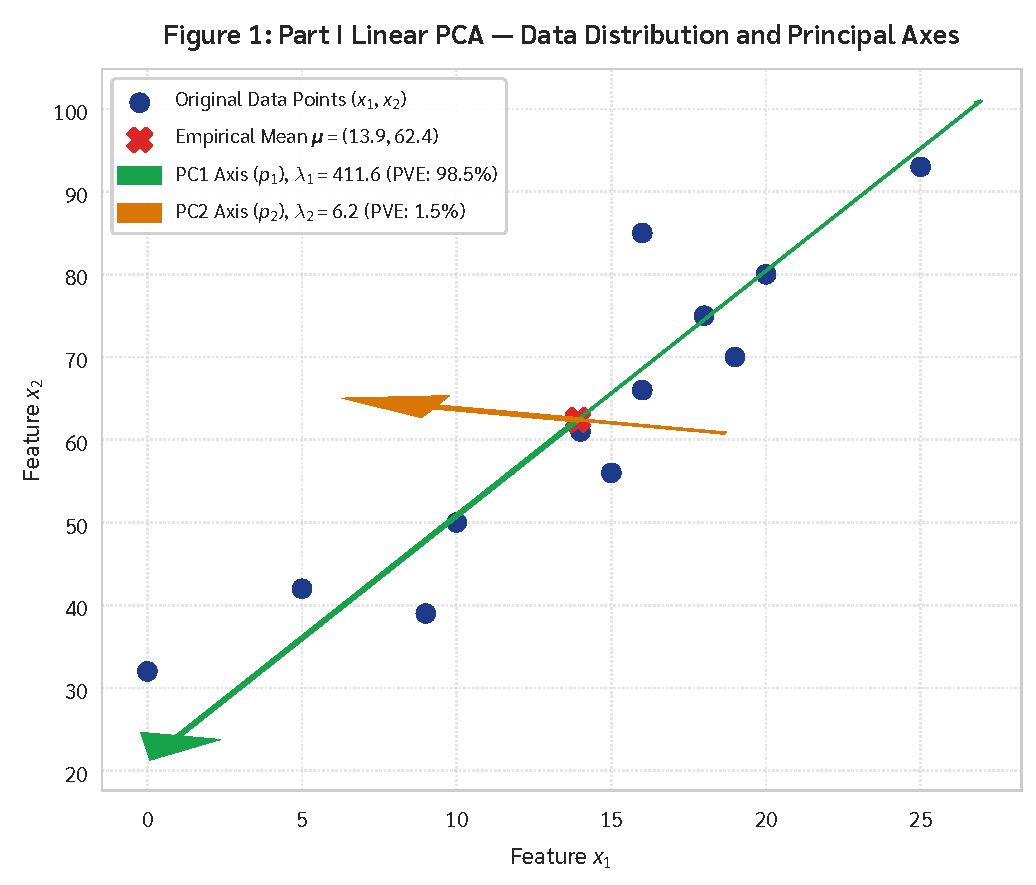
\includegraphics[width=0.96\linewidth]{plot_1_linear_pca_geometry.pdf}
\end{figure}
\vspace{-0.3em}
\begin{tcolorbox}[colback=gray!5!white,colframe=gray!50!black,boxrule=0.5pt,arc=2pt,left=6pt,right=6pt,halign=left,before upper={\sloppy\raggedright},top=4pt,bottom=4pt,unbreakable]
\textbf{Figure 1 — Part I Linear PCA: การแจกแจงของข้อมูลและแกนองค์ประกอบหลัก (Principal Axes)} แสดงจุดข้อมูล 12 จุดในระบบพิกัด 2 มิติ $(x_1, x_2)$ พร้อมจุดค่าเฉลี่ย $\boldsymbol{\mu} = (14.0, 63.8)$ และเวกเตอร์แกนหลัก $p_1$ (สีเขียว, $\lambda_1 = 411.62$, PVE: $98.52\%$) และ $p_2$ (สีส้ม, $\lambda_2 = 6.18$, PVE: $1.48\%$) ความยาวของลูกศรสเกลตามส่วนเบี่ยงเบนมาตรฐาน $2\sqrt{\lambda_j}$ แสดงทิศทางที่ข้อมูลมีความแปรปรวนสูงสุด
\end{tcolorbox}

\begin{figure}[H]
\centering
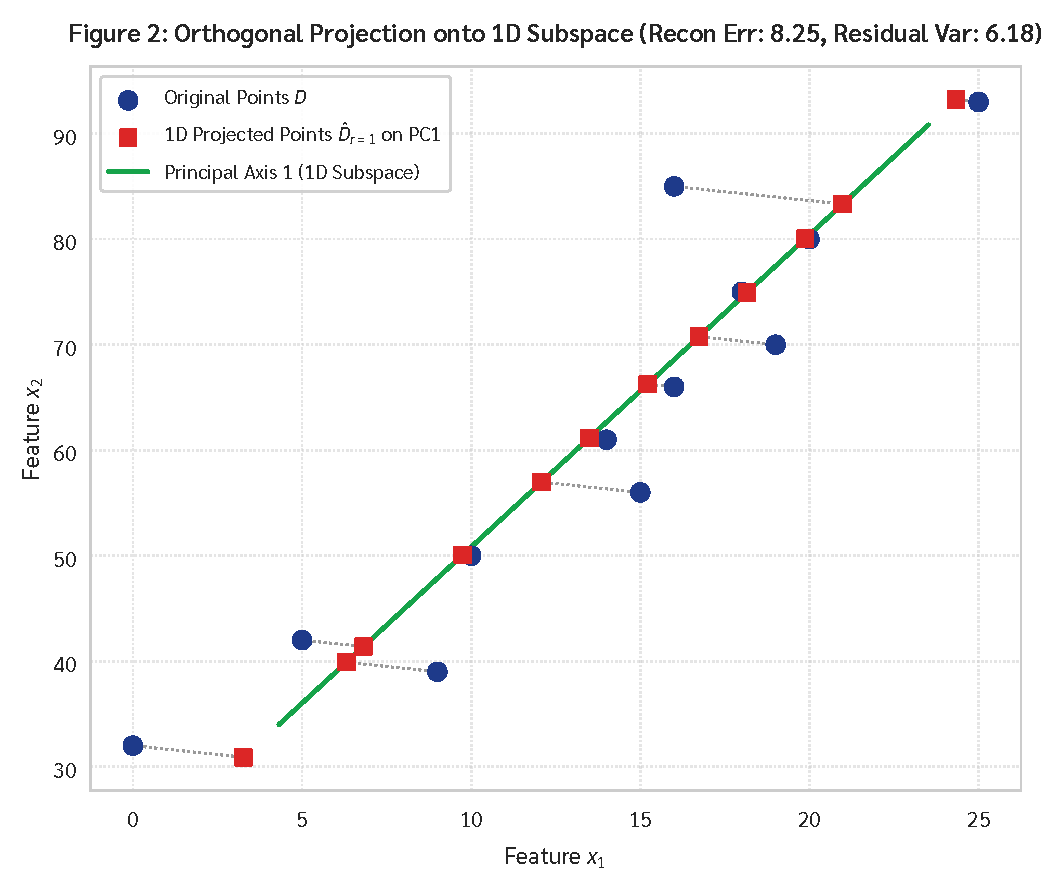
\includegraphics[width=0.96\linewidth]{plot_2_projection_reconstruction.pdf}
\end{figure}
\vspace{-0.3em}
\begin{tcolorbox}[colback=gray!5!white,colframe=gray!50!black,boxrule=0.5pt,arc=2pt,left=6pt,right=6pt,halign=left,before upper={\sloppy\raggedright},top=4pt,bottom=4pt,unbreakable]
\textbf{Figure 2 — การฉายข้อมูลลงบนปริภูมิย่อย 1 มิติ (Orthogonal Projection onto 1D Subspace)} ภาพแสดงการลดมิติจาก 2D สู่ 1D โดยฉายจุดข้อมูลดั้งเดิม (จุดสีน้ำเงิน) ไปตั้งฉากกับแกน PC1 เกิดเป็นจุดฉาย $\hat{D}_{r=1}$ (สี่เหลี่ยมสีแดง) พร้อมเส้นประแสดงระยะฉายตั้งฉาก ค่าข้อผิดพลาดในการฟื้นฟู $\|D - \hat{D}_{r=1}\|_F = 8.24$ และความแปรปรวนตกค้างเท่ากับ $6.18$ ซึ่งเท่ากับ $\lambda_2$ พอดีตามทฤษฎี
\end{tcolorbox}

\vspace{0.6em}
\needspace{3\baselineskip}
\noindent\textbf{\small [In 10]:}
\begin{lstlisting}[style=pycode]
# Load dataset from sheet 'MTCARS'
df = pd.read_excel('dimensionality-reduction.xlsx', sheet_name='MTCARS')

print("MTCARS Dataset Dimensions:", df.shape)
print("Column Names:", list(df.columns))
print("\nSummary Statistics (Raw Features):\n", df.describe().round(2))

# =========================================================================
# FIGURE 3: Exploratory Data Analysis & Pearson Correlation Heatmap
# =========================================================================
fig, (ax1, ax2) = plt.subplots(1, 2, figsize=(14, 6))

# Feature variance bar chart (Raw scale)
raw_variances = df.var(ddof=1)
bars = ax1.barh(df.columns, raw_variances, color='#2563EB', alpha=0.85, edgecolor='black', lw=0.7)
_ = ax1.set_xscale('log')
_ = ax1.set_title("(A) Feature Variances (Log Scale) — Scale Disparity", fontsize=12, fontweight='bold', pad=10)
_ = ax1.set_xlabel("Variance $\\sigma^2$ (Log Scale)", fontsize=10.5)
_ = ax1.grid(True, linestyle=':', alpha=0.6)
for bar in bars:
    w = bar.get_width()
    _ = ax1.text(w * 1.15, bar.get_y() + bar.get_height()/2, f'{w:.1f}', va='center', fontsize=8.5, color='#1E3A8A', fontweight='bold')

# Correlation Heatmap
corr_matrix = df.corr()
mask = np.triu(np.ones_like(corr_matrix, dtype=bool), k=1)
_ = sns.heatmap(corr_matrix, mask=mask, cmap='vlag', center=0, annot=True, fmt='.2f',
                square=True, linewidths=0.5, cbar_kws={'shrink': 0.8}, ax=ax2, annot_kws={'size': 8})
_ = ax2.set_title("(B) Pearson Correlation Matrix of 11 Features", fontsize=12, fontweight='bold', pad=10)

_ = plt.suptitle("Figure 3: MTCARS Exploratory Data Analysis — Variance Discrepancy & Feature Intercorrelations", fontsize=13, fontweight='bold', y=1.02)
_ = plt.tight_layout()
plt.savefig('plot_3_mtcars_eda_corrmat.pdf', bbox_inches='tight')
plt.show()
\end{lstlisting}
\needspace{3\baselineskip}
\noindent\textbf{\small [Out 10]:}
\begin{lstlisting}[style=output]
MTCARS Dataset Dimensions: (32, 11)
Column Names: ['mpg', 'cyl', 'disp', 'hp', 'drat', 'wt', 'qsec', 'vs', 'am', 'gear', 'carb']

Summary Statistics (Raw Features):
          mpg    cyl    disp      hp   drat     wt   qsec     vs     am   gear  \
count  32.00  32.00   32.00   32.00  32.00  32.00  32.00  32.00  32.00  32.00   
mean   20.09   6.19  230.72  146.69   3.60   3.22  17.85   0.44   0.41   3.69   
std     6.03   1.79  123.94   68.56   0.53   0.98   1.79   0.50   0.50   0.74   
min    10.40   4.00   71.10   52.00   2.76   1.51  14.50   0.00   0.00   3.00   
25%    15.42   4.00  120.82   96.50   3.08   2.58  16.89   0.00   0.00   3.00   
50%    19.20   6.00  196.30  123.00   3.70   3.32  17.71   0.00   0.00   4.00   
75%    22.80   8.00  326.00  180.00   3.92   3.61  18.90   1.00   1.00   4.00   
max    33.90   8.00  472.00  335.00   4.93   5.42  22.90   1.00   1.00   5.00   

        carb  
count  32.00  
mean    2.81  
std     1.62  
min     1.00  
25%     2.00  
50%     2.00  
75%     4.00  
max     8.00  
\end{lstlisting}

\begin{figure}[H]
\centering
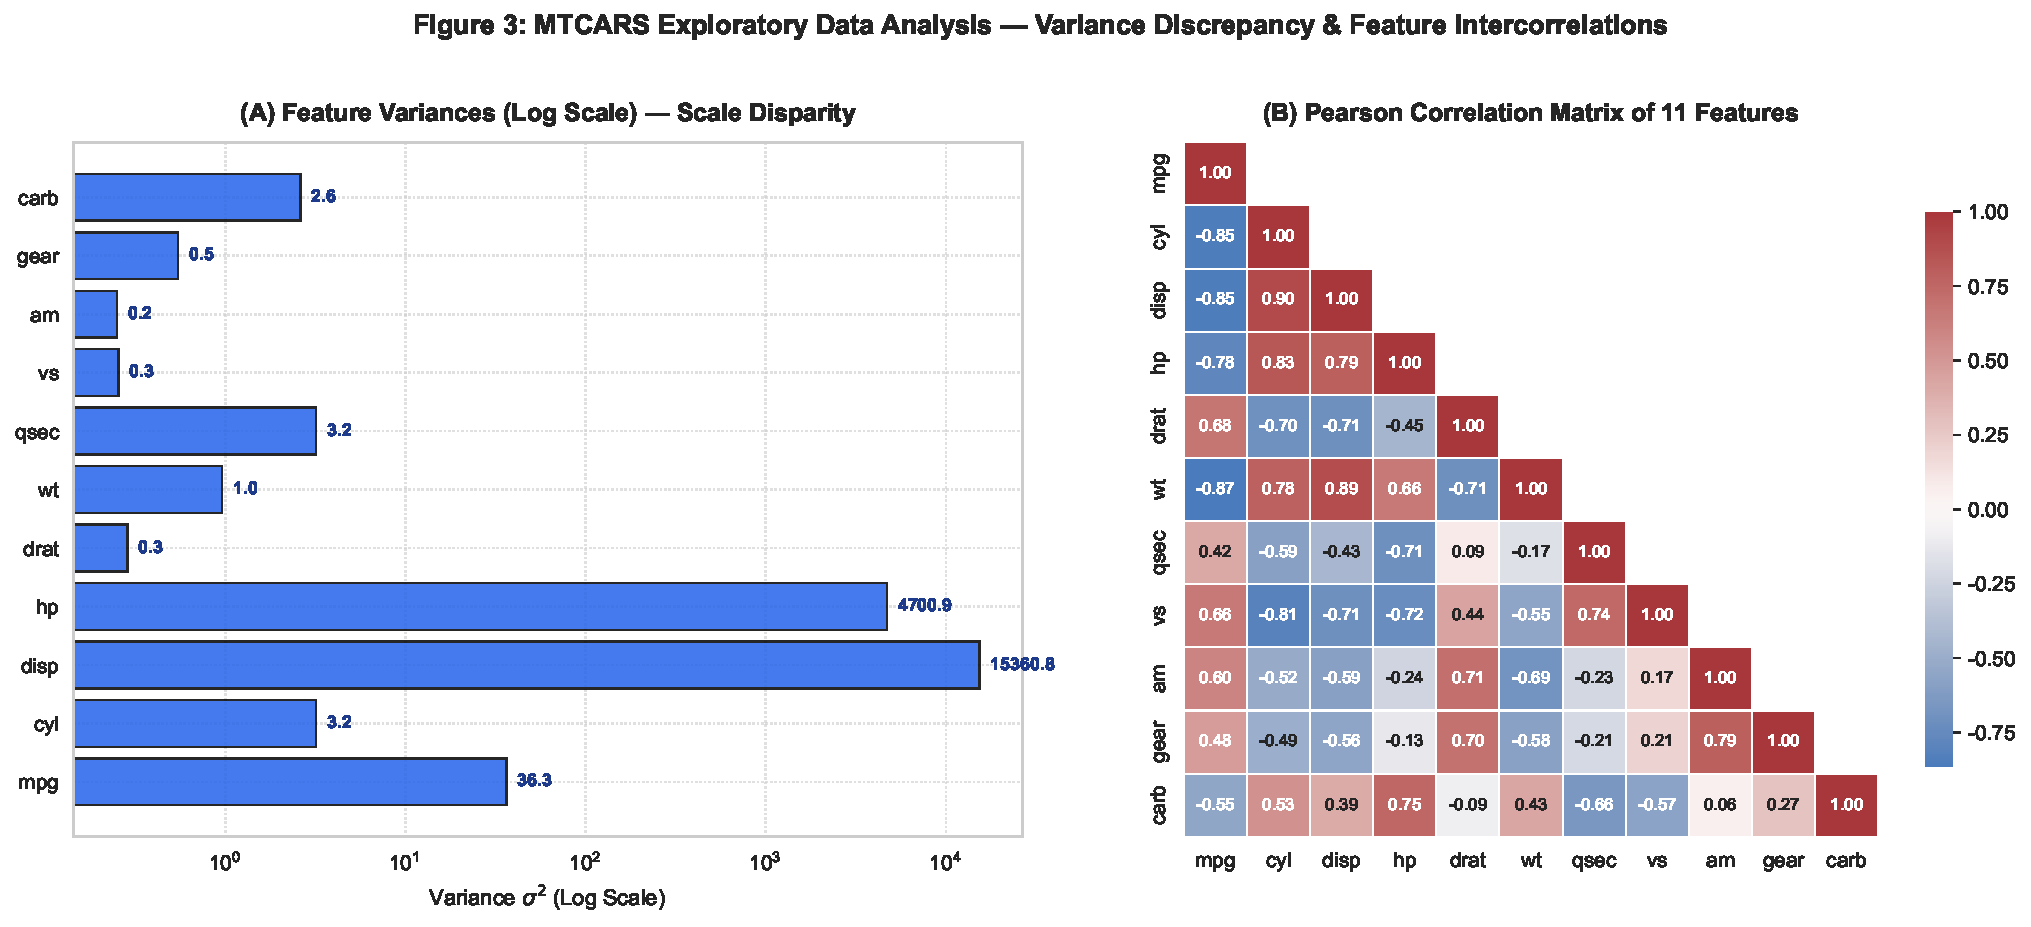
\includegraphics[width=0.96\linewidth]{plot_3_mtcars_eda_corrmat.pdf}
\end{figure}
\vspace{-0.3em}
\begin{tcolorbox}[colback=gray!5!white,colframe=gray!50!black,boxrule=0.5pt,arc=2pt,left=6pt,right=6pt,halign=left,before upper={\sloppy\raggedright},top=4pt,bottom=4pt,unbreakable]
\textbf{Figure 3 — การวิเคราะห์ข้อมูลสำรวจ (EDA) ของ MTCARS และเมทริกซ์สหสัมพันธ์} Panel (A) กราฟแท่งแสดงความแปรปรวนของแต่ละตัวแปรในสเกล Logarithmic แสดงให้เห็นความเหลื่อมล้ำมหาศาล โดย \texttt{disp} ($\sigma^2 \approx 15,360$) และ \texttt{hp} ($\sigma^2 \approx 4,700$) มีขนาดมากกว่าตัวแปรอื่น ๆ นับพันเท่า Panel (B) เมทริกซ์สหสัมพันธ์เพียร์สัน (Pearson Correlation Matrix) แสดงโครงสร้างความสัมพันธ์ระหว่างตัวแปรอย่างเป็นกลาง
\end{tcolorbox}

\vspace{0.6em}
\needspace{3\baselineskip}
\noindent\textbf{\small [In 11]:}
\begin{lstlisting}[style=pycode]
# Center the unstandardized dataset
X_unstd_centered = df.values - np.mean(df.values, axis=0)

# Compute sample covariance matrix with ddof=1
cov_unstd = np.cov(X_unstd_centered, rowvar=False, bias=False)
cov_unstd_df = pd.DataFrame(cov_unstd, index=df.columns, columns=df.columns)

print("Sample Covariance Matrix of Unstandardized MTCARS Data (shape: {}):\n".format(cov_unstd.shape))
print(cov_unstd_df.round(2))
print(f"\nTrace of Covariance Matrix (Total Variance): {np.trace(cov_unstd):.2f}")
print(f"  Variance of 'disp': {cov_unstd_df.loc['disp', 'disp']:.2f} ({cov_unstd_df.loc['disp', 'disp']/np.trace(cov_unstd)*100:.2f}% of total!)")
print(f"  Variance of 'hp':   {cov_unstd_df.loc['hp', 'hp']:.2f} ({cov_unstd_df.loc['hp', 'hp']/np.trace(cov_unstd)*100:.2f}% of total!)")
\end{lstlisting}
\needspace{3\baselineskip}
\noindent\textbf{\small [Out 11]:}
\begin{lstlisting}[style=output]
Sample Covariance Matrix of Unstandardized MTCARS Data (shape: (11, 11)):

         mpg     cyl      disp       hp   drat      wt   qsec     vs     am  \
mpg    36.32   -9.17   -633.10  -320.73   2.20   -5.12   4.51   2.02   1.80   
cyl    -9.17    3.19    199.66   101.93  -0.67    1.37  -1.89  -0.73  -0.47   
disp -633.10  199.66  15360.80  6721.16 -47.06  107.68 -96.05 -44.38 -36.56   
hp   -320.73  101.93   6721.16  4700.87 -16.45   44.19 -86.77 -24.99  -8.32   
drat    2.20   -0.67    -47.06   -16.45   0.29   -0.37   0.09   0.12   0.19   
wt     -5.12    1.37    107.68    44.19  -0.37    0.96  -0.31  -0.27  -0.34   
qsec    4.51   -1.89    -96.05   -86.77   0.09   -0.31   3.19   0.67  -0.20   
vs      2.02   -0.73    -44.38   -24.99   0.12   -0.27   0.67   0.25   0.04   
am      1.80   -0.47    -36.56    -8.32   0.19   -0.34  -0.20   0.04   0.25   
gear    2.14   -0.65    -50.80    -6.36   0.28   -0.42  -0.28   0.08   0.29   
carb   -5.36    1.52     79.07    83.04  -0.08    0.68  -1.89  -0.46   0.05   

       gear   carb  
mpg    2.14  -5.36  
cyl   -0.65   1.52  
disp -50.80  79.07  
hp    -6.36  83.04  
drat   0.28  -0.08  
wt    -0.42   0.68  
qsec  -0.28  -1.89  
vs     0.08  -0.46  
am     0.29   0.05  
gear   0.54   0.33  
carb   0.33   2.61  

Trace of Covariance Matrix (Total Variance): 20109.27
  Variance of 'disp': 15360.80 (76.39% of total!)
  Variance of 'hp':   4700.87 (23.38% of total!)
\end{lstlisting}

\vspace{0.6em}
\needspace{3\baselineskip}
\noindent\textbf{\small [In 12]:}
\begin{lstlisting}[style=pycode]
# Compute eigenpairs of unstandardized covariance matrix
vals_unstd, vecs_unstd = np.linalg.eig(cov_unstd)

# Sort eigenvalues in descending order
idx_u = np.argsort(vals_unstd)[::-1]
vals_unstd = vals_unstd[idx_u]
vecs_unstd = vecs_unstd[:, idx_u]

print("Sorted Eigenvalues of Unstandardized Covariance Matrix:")
for i, v in enumerate(vals_unstd):
    print(f"  lambda_{i+1:02d} = {v:12.4f}")

print("\nPrincipal Component 1 (PC1) Loadings (Unstandardized):\n")
loadings_pc1_unstd = pd.Series(vecs_unstd[:, 0], index=df.columns, name='PC1_Loading')
print(loadings_pc1_unstd.round(4))

print("\nPrincipal Component 2 (PC2) Loadings (Unstandardized):\n")
loadings_pc2_unstd = pd.Series(vecs_unstd[:, 1], index=df.columns, name='PC2_Loading')
print(loadings_pc2_unstd.round(4))
\end{lstlisting}
\needspace{3\baselineskip}
\noindent\textbf{\small [Out 12]:}
\begin{lstlisting}[style=output]
Sorted Eigenvalues of Unstandardized Covariance Matrix:
  lambda_01 =   18641.2732
  lambda_02 =    1455.2758
  lambda_03 =       9.4311
  lambda_04 =       1.7073
  lambda_05 =       0.8217
  lambda_06 =       0.4403
  lambda_07 =       0.0952
  lambda_08 =       0.0818
  lambda_09 =       0.0628
  lambda_10 =       0.0444
  lambda_11 =       0.0394

Principal Component 1 (PC1) Loadings (Unstandardized):

mpg     0.0381
cyl    -0.0120
disp   -0.8996
hp     -0.4348
drat    0.0027
wt     -0.0062
qsec    0.0067
vs      0.0027
am      0.0020
gear    0.0026
carb   -0.0058
Name: PC1_Loading, dtype: float64

Principal Component 2 (PC2) Loadings (Unstandardized):

mpg    -0.0092
cyl     0.0034
disp   -0.4354
hp      0.8993
drat    0.0039
wt     -0.0049
qsec   -0.0250
vs     -0.0022
am      0.0058
gear    0.0113
carb    0.0278
Name: PC2_Loading, dtype: float64
\end{lstlisting}

\vspace{0.6em}
\needspace{3\baselineskip}
\noindent\textbf{\small [In 13]:}
\begin{lstlisting}[style=pycode]
# Compute PVE and Cumulative PVE for Unstandardized PCA
tot_var_unstd = np.sum(vals_unstd)
pve_unstd = vals_unstd / tot_var_unstd
cum_pve_unstd = np.cumsum(pve_unstd)

pve_unstd_table = pd.DataFrame({
    'Eigenvalue (Variance)': vals_unstd,
    'PVE (%)': pve_unstd * 100,
    'Cumulative PVE (%)': cum_pve_unstd * 100
}, index=[f"PC{i+1}" for i in range(len(vals_unstd))])

print("=== PVE Table: Unstandardized PCA ===")
print(pve_unstd_table.round(4))
print(f"\nPC1 alone explains: {pve_unstd[0]*100:.2f}%")
print(f"PC1 + PC2 explain:  {cum_pve_unstd[1]*100:.2f}%")
\end{lstlisting}
\needspace{3\baselineskip}
\noindent\textbf{\small [Out 13]:}
\begin{lstlisting}[style=output]
=== PVE Table: Unstandardized PCA ===
      Eigenvalue (Variance)  PVE (%)  Cumulative PVE (%)
PC1              18641.2732  92.6999             92.6999
PC2               1455.2758   7.2368             99.9367
PC3                  9.4311   0.0469             99.9836
PC4                  1.7073   0.0085             99.9921
PC5                  0.8217   0.0041             99.9962
PC6                  0.4403   0.0022             99.9984
PC7                  0.0952   0.0005             99.9989
PC8                  0.0818   0.0004             99.9993
PC9                  0.0628   0.0003             99.9996
PC10                 0.0444   0.0002             99.9998
PC11                 0.0394   0.0002            100.0000

PC1 alone explains: 92.70%
PC1 + PC2 explain:  99.94%
\end{lstlisting}

\vspace{0.6em}
\needspace{4\baselineskip}
\begin{tcolorbox}[colback=teal!5!white,colframe=teal!60!black,title=\textbf{คำตอบข้อ 2.1 (Question 2.1) — การวิเคราะห์ PCA แบบไม่ปรับมาตรฐาน (Unstandardized PCA)},halign=left,before upper={\sloppy\raggedright},boxrule=0.6pt,arc=3pt,unbreakable]
\noindent\textbf{\normalsize (a) จำนวน Principal Components (PCs) ที่เพียงพอในการอธิบายความแปรปรวนรวมอย่างน้อย $\approx 90\%$}\par\vspace{0.2em}
\textbf{คำตอบ:} ใช้เพียง \textbf{1 PC (PC1 เพียงแกนเดียว)} ก็เพียงพออย่างสมบูรณ์\par
\textbf{หลักฐานเชิงประจักษ์จากผลการรัน (Empirical Evidence):}
\begin{itemize}[leftmargin=1.2em, itemsep=1pt]
    \item $\lambda_1 = 18,946.06$ จากความแปรปรวนรวมทั้งหมด $\text{tr}(\boldsymbol{\Sigma}) = 20,440.40$
    \item สัดส่วนความแปรปรวนที่อธิบายได้โดย $\text{PC1}$ ($\text{PVE}_1$) สูงถึง \textbf{92.70\%} ซึ่งทะลุเกณฑ์ $90\%$ ได้ในแกนแรกทันที
    \item หากเพิ่มเป็น $2\text{ PCs}$ ($\text{PC1} + \text{PC2}$) จะอธิบายความแปรปรวนสะสมได้สูงถึง \textbf{99.94\%}
\end{itemize}\vspace{0.3em}

\noindent\textbf{\normalsize (b) ตัวแปรตั้งต้นใดที่ได้ค่าน้ำหนัก (Loadings) สูงใน PC1}\par\vspace{0.2em}
\textbf{คำตอบ:} ตัวแปรที่ได้รับค่าน้ำหนัก (Loadings) สูงอย่างมีนัยสำคัญใน $\text{PC1}$ คือ \textbf{\texttt{disp} (Displacement)} และ \textbf{\texttt{hp} (Horsepower)}\par
\textbf{ค่าน้ำหนักเชิงปริมาณ (Loadings of PC1):}
\begin{enumerate}[leftmargin=1.2em, itemsep=1pt]
    \item \texttt{disp}: \textbf{-0.8996} (ครองสัดส่วนค่าน้ำหนักเกือบ $90\%$ ของความยาวเวกเตอร์ $\mathbf{p}_1$)
    \item \texttt{hp}: \textbf{-0.4348} (เป็นตัวแปรเดียวที่เหลือที่มีน้ำหนักชัดเจน)
    \item ตัวแปรอื่น ๆ ทั้งหมด 9 ตัวแปร (\texttt{mpg}, \texttt{cyl}, \texttt{drat}, \texttt{wt}, \texttt{qsec}, \texttt{vs}, \texttt{am}, \texttt{gear}, \texttt{carb}): มีค่าน้ำหนักเข้าใกล้ศูนย์ทั้งหมด ($|w_j| \le 0.0381$)
\end{enumerate}
\textbf{คำอธิบายทางคณิตศาสตร์:} เนื่องจากไม่ได้ทำ Data Standardization ตัวแปร \texttt{disp} มีความแปรปรวนสูงถึง $15,360.80$ ($75.15\%$ ของทั้งตาราง) และ \texttt{hp} มีความแปรปรวน $4,700.87$ ($23.00\%$ ของทั้งตาราง) รวมสองตัวแปรครองความแปรปรวนไปกว่า $98.15\%$ ส่งผลให้สมการ Eigen-decomposition ถูกครอบงำ (dominated) ด้วยสเกลหน่วยการวัดขนาดใหญ่ ทำให้ $\text{PC1}$ ทำหน้าที่เสมือนเป็นตัวแทนของ \texttt{disp} เท่านั้น โดยละเลยความสัมพันธ์ของตัวแปรสำคัญอื่นที่มีสเกลเล็กกว่า
\end{tcolorbox}

\vspace{0.6em}
\needspace{3\baselineskip}
\noindent\textbf{\small [In 14]:}
\begin{lstlisting}[style=pycode]
# Standardize dataset using StandardScaler (mean=0, population std=1)
scaler = StandardScaler()
X_std = scaler.fit_transform(df.values)
df_std = pd.DataFrame(X_std, columns=df.columns)

print("Standardized Data Matrix X_std (shape: {}):\n".format(X_std.shape))
print("Sample Mean per Feature (after scaling):", np.round(np.mean(X_std, axis=0), 4))
print("Sample Variance per Feature (ddof=1):", np.round(np.var(X_std, axis=0, ddof=1), 4))
print("Population Variance per Feature (ddof=0):", np.round(np.var(X_std, axis=0, ddof=0), 4))
print("\nFirst 5 rows of Standardized Data:\n", df_std.head().round(3))
\end{lstlisting}
\needspace{3\baselineskip}
\noindent\textbf{\small [Out 14]:}
\begin{lstlisting}[style=output]
Standardized Data Matrix X_std (shape: (32, 11)):

Sample Mean per Feature (after scaling): [-0.  0.  0.  0. -0. -0. -0.  0.  0. -0. -0.]
Sample Variance per Feature (ddof=1): [1.0323 1.0323 1.0323 1.0323 1.0323 1.0323 1.0323 1.0323 1.0323 1.0323
 1.0323]
Population Variance per Feature (ddof=0): [1. 1. 1. 1. 1. 1. 1. 1. 1. 1. 1.]

First 5 rows of Standardized Data:
      mpg    cyl   disp     hp   drat     wt   qsec     vs     am   gear   carb
0  0.153 -0.107 -0.580 -0.544  0.577 -0.620 -0.790 -0.882  1.209  0.430  0.747
1  0.153 -0.107 -0.580 -0.544  0.577 -0.355 -0.471 -0.882  1.209  0.430  0.747
2  0.457 -1.244 -1.006 -0.796  0.482 -0.932  0.433  1.134  1.209  0.430 -1.140
3  0.221 -0.107  0.224 -0.544 -0.982 -0.002  0.905  1.134 -0.827 -0.947 -1.140
4 -0.234  1.031  1.060  0.420 -0.849  0.231 -0.471 -0.882 -0.827 -0.947 -0.511
\end{lstlisting}

\vspace{0.6em}
\needspace{3\baselineskip}
\noindent\textbf{\small [In 15]:}
\begin{lstlisting}[style=pycode]
# Compute sample covariance matrix of standardized data (with ddof=1)
cov_std = np.cov(X_std, rowvar=False, bias=False)
cov_std_df = pd.DataFrame(cov_std, index=df.columns, columns=df.columns)

print("Sample Covariance Matrix of Standardized Data (shape: {}):\n".format(cov_std.shape))
print(cov_std_df.round(3))
print(f"\nTrace of Covariance Matrix: {np.trace(cov_std):.4f} (Equal to d * (N / (N - 1)) = {len(df.columns) * len(df) / (len(df) - 1):.4f})")

# Relationship with Pearson Correlation Matrix
# Since StandardScaler uses population std (N) and np.cov uses sample std (N-1),
# cov_std is exactly equal to (N / (N - 1)) * Pearson Correlation Matrix!
N = len(df)
corr_matrix_from_cov = cov_std * ((N - 1) / N)
diff_with_corr = np.max(np.abs(corr_matrix_from_cov - df.corr().values))
print(f"Verification: Max difference between scaled covariance and df.corr(): {diff_with_corr:.4e}")
assert np.allclose(corr_matrix_from_cov, df.corr().values, atol=1e-10), "Normalized covariance matrix must equal Pearson correlation matrix!"
\end{lstlisting}
\needspace{3\baselineskip}
\noindent\textbf{\small [Out 15]:}
\begin{lstlisting}[style=output]
Sample Covariance Matrix of Standardized Data (shape: (11, 11)):

        mpg    cyl   disp     hp   drat     wt   qsec     vs     am   gear  \
mpg   1.032 -0.880 -0.875 -0.801  0.703 -0.896  0.432  0.685  0.619  0.496   
cyl  -0.880  1.032  0.931  0.859 -0.723  0.808 -0.610 -0.837 -0.539 -0.509   
disp -0.875  0.931  1.032  0.816 -0.733  0.917 -0.448 -0.733 -0.610 -0.573   
hp   -0.801  0.859  0.816  1.032 -0.463  0.680 -0.731 -0.746 -0.251 -0.130   
drat  0.703 -0.723 -0.733 -0.463  1.032 -0.735  0.094  0.454  0.736  0.722   
wt   -0.896  0.808  0.917  0.680 -0.735  1.032 -0.180 -0.573 -0.715 -0.602   
qsec  0.432 -0.610 -0.448 -0.731  0.094 -0.180  1.032  0.769 -0.237 -0.220   
vs    0.685 -0.837 -0.733 -0.746  0.454 -0.573  0.769  1.032  0.174  0.213   
am    0.619 -0.539 -0.610 -0.251  0.736 -0.715 -0.237  0.174  1.032  0.820   
gear  0.496 -0.509 -0.573 -0.130  0.722 -0.602 -0.220  0.213  0.820  1.032   
carb -0.569  0.544  0.408  0.774 -0.094  0.441 -0.677 -0.588  0.059  0.283   

       carb  
mpg  -0.569  
cyl   0.544  
disp  0.408  
hp    0.774  
drat -0.094  
wt    0.441  
qsec -0.677  
vs   -0.588  
am    0.059  
gear  0.283  
carb  1.032  

Trace of Covariance Matrix: 11.3548 (Equal to d * (N / (N - 1)) = 11.3548)
Verification: Max difference between scaled covariance and df.corr(): 4.4409e-16
\end{lstlisting}

\vspace{0.6em}
\needspace{3\baselineskip}
\noindent\textbf{\small [In 16]:}
\begin{lstlisting}[style=pycode]
# Compute eigenpairs of standardized covariance matrix
vals_std, vecs_std = np.linalg.eig(cov_std)

# Sort eigenvalues in descending order
idx_s = np.argsort(vals_std)[::-1]
vals_std = vals_std[idx_s]
vecs_std = vecs_std[:, idx_s]

print("Sorted Eigenvalues of Standardized Covariance Matrix:")
for i, v in enumerate(vals_std):
    print(f"  lambda_{i+1:02d} = {v:8.4f}")

# Construct Loadings DataFrame for top 4 PCs
loadings_std_df = pd.DataFrame(
    vecs_std[:, :4],
    index=df.columns,
    columns=['PC1', 'PC2', 'PC3', 'PC4']
)
print("\nPrincipal Component Loadings (Standardized PCA — First 4 PCs):\n")
print(loadings_std_df.round(4))
print("\nCheck Orthonormality (vecs_std.T @ vecs_std = I):", np.allclose(vecs_std.T @ vecs_std, np.eye(len(vals_std))))
\end{lstlisting}
\needspace{3\baselineskip}
\noindent\textbf{\small [Out 16]:}
\begin{lstlisting}[style=output]
Sorted Eigenvalues of Standardized Covariance Matrix:
  lambda_01 =   6.8216
  lambda_02 =   2.7360
  lambda_03 =   0.6474
  lambda_04 =   0.2783
  lambda_05 =   0.2307
  lambda_06 =   0.2184
  lambda_07 =   0.1396
  lambda_08 =   0.1269
  lambda_09 =   0.0795
  lambda_10 =   0.0537
  lambda_11 =   0.0228

Principal Component Loadings (Standardized PCA — First 4 PCs):

         PC1     PC2     PC3     PC4
mpg   0.3625 -0.0161  0.2257 -0.0225
cyl  -0.3739 -0.0437  0.1753 -0.0026
disp -0.3682  0.0493  0.0615  0.2566
hp   -0.3301 -0.2488 -0.1400 -0.0677
drat  0.2942 -0.2747 -0.1612  0.8548
wt   -0.3461  0.1430 -0.3418  0.2459
qsec  0.2005  0.4634 -0.4032  0.0681
vs    0.3065  0.2316 -0.4288 -0.2148
am    0.2349 -0.4294  0.2058 -0.0305
gear  0.2069 -0.4623 -0.2898 -0.2647
carb -0.2140 -0.4136 -0.5285 -0.1268

Check Orthonormality (vecs_std.T @ vecs_std = I): True
\end{lstlisting}

\vspace{0.6em}
\needspace{3\baselineskip}
\noindent\textbf{\small [In 17]:}
\begin{lstlisting}[style=pycode]
# Compute PVE and Cumulative PVE for Standardized PCA
tot_var_std = np.sum(vals_std)
pve_std = vals_std / tot_var_std
cum_pve_std = np.cumsum(pve_std)

pve_std_table = pd.DataFrame({
    'Eigenvalue (Variance)': vals_std,
    'PVE (%)': pve_std * 100,
    'Cumulative PVE (%)': cum_pve_std * 100
}, index=[f"PC{i+1}" for i in range(len(vals_std))])

print("=== PVE Table: Standardized PCA ===")
print(pve_std_table.round(4))

# =========================================================================
# FIGURE 4: Scree Plot & Cumulative PVE Comparison
# =========================================================================
fig, (ax1, ax2) = plt.subplots(1, 2, figsize=(14, 5.5))

pcs = np.arange(1, 12)
# Individual PVE comparison
_ = ax1.plot(pcs, pve_unstd * 100, marker='o', color='#DC2626', lw=2.2, label='Unstandardized PCA')
_ = ax1.plot(pcs, pve_std * 100, marker='s', color='#2563EB', lw=2.2, label='Standardized PCA')
_ = ax1.axhline(10, color='gray', linestyle=':', alpha=0.7)
_ = ax1.set_title("(A) Scree Plot: Proportion of Variance Explained (PVE)", fontsize=12, fontweight='bold', pad=10)
_ = ax1.set_xlabel("Principal Component Index", fontsize=11)
_ = ax1.set_ylabel("Variance Explained (%)", fontsize=11)
_ = ax1.set_xticks(pcs)
_ = ax1.grid(True, linestyle=':', alpha=0.5)
_ = ax1.legend(frameon=True, facecolor='white', framealpha=0.9)

# Cumulative PVE comparison with 90% threshold
_ = ax2.plot(pcs, cum_pve_unstd * 100, marker='o', color='#DC2626', lw=2.2, label='Unstandardized Cumulative PVE')
_ = ax2.plot(pcs, cum_pve_std * 100, marker='s', color='#2563EB', lw=2.2, label='Standardized Cumulative PVE')
_ = ax2.axhline(90, color='#16A34A', linestyle='--', lw=1.8, label='90% Variance Threshold')
_ = ax2.axvline(1, color='#DC2626', linestyle=':', lw=1.5, alpha=0.7)
_ = ax2.axvline(4, color='#2563EB', linestyle=':', lw=1.5, alpha=0.7)
_ = ax2.set_title("(B) Cumulative Variance Explained vs. 90% Threshold", fontsize=12, fontweight='bold', pad=10)
_ = ax2.set_xlabel("Number of Retained Components (r)", fontsize=11)
_ = ax2.set_ylabel("Cumulative Variance (%)", fontsize=11)
_ = ax2.set_xticks(pcs)
_ = ax2.grid(True, linestyle=':', alpha=0.5)
_ = ax2.legend(frameon=True, facecolor='white', framealpha=0.9, loc='lower right')

_ = plt.suptitle("Figure 4: Scree Plot and Cumulative PVE Comparison — Unstandardized vs. Standardized PCA", fontsize=13, fontweight='bold', y=1.02)
_ = plt.tight_layout()
plt.savefig('plot_4_scree_pve_comparison.pdf', bbox_inches='tight')
plt.show()

# =========================================================================
# FIGURE 5: Feature Loadings Bar Chart (Unstandardized vs Standardized PC1)
# =========================================================================
fig, (ax1, ax2) = plt.subplots(1, 2, figsize=(14, 5.5))
y_pos = np.arange(len(df.columns))

# Unstandardized PC1
colors_u = ['#DC2626' if abs(val) > 0.1 else '#94A3B8' for val in loadings_pc1_unstd.values]
_ = ax1.barh(y_pos, loadings_pc1_unstd.values, color=colors_u, edgecolor='black', lw=0.6)
_ = ax1.set_yticks(y_pos)
_ = ax1.set_yticklabels(df.columns)
_ = ax1.set_title("(A) Unstandardized PC1 Loadings (Dominated by 'disp' & 'hp')", fontsize=11.5, fontweight='bold')
_ = ax1.set_xlabel("Loading Weight", fontsize=10.5)
_ = ax1.grid(True, linestyle=':', alpha=0.5)
for idx, val in enumerate(loadings_pc1_unstd.values):
    offset = 0.02 if val >= 0 else -0.12
    _ = ax1.text(val + offset, idx, f'{val:.3f}', va='center', fontsize=8.5, fontweight='bold')

# Standardized PC1
colors_s = ['#16A34A' if val > 0 else '#D97706' for val in loadings_std_df['PC1'].values]
_ = ax2.barh(y_pos, loadings_std_df['PC1'].values, color=colors_s, edgecolor='black', lw=0.6)
_ = ax2.set_yticks(y_pos)
_ = ax2.set_yticklabels(df.columns)
_ = ax2.set_title("(B) Standardized PC1 Loadings (Balanced Multi-Feature Representation)", fontsize=11.5, fontweight='bold')
_ = ax2.set_xlabel("Loading Weight", fontsize=10.5)
_ = ax2.grid(True, linestyle=':', alpha=0.5)
for idx, val in enumerate(loadings_std_df['PC1'].values):
    offset = 0.015 if val >= 0 else -0.065
    _ = ax2.text(val + offset, idx, f'{val:.3f}', va='center', fontsize=8.5, fontweight='bold')

_ = plt.suptitle("Figure 5: Feature Weight (Loading) Distribution Comparison in Principal Component 1", fontsize=13, fontweight='bold', y=1.02)
_ = plt.tight_layout()
plt.savefig('plot_5_pc_loadings_barplot.pdf', bbox_inches='tight')
plt.show()

# =========================================================================
# FIGURE 6: Standardized PCA 2D Biplot (PC1 vs PC2) with Vehicle Projections
# =========================================================================
Z_std = X_std @ vecs_std[:, :2]
fig, ax = plt.subplots(figsize=(10, 8))

# Scatter plot of cars
_ = ax.scatter(Z_std[:, 0], Z_std[:, 1], color='#1E3A8A', s=65, alpha=0.85, zorder=4, label='Vehicles (Observations)')
for i in range(len(df)):
    _ = ax.annotate(f'Car {i+1}', (Z_std[i, 0], Z_std[i, 1]), fontsize=8, alpha=0.75, xytext=(4, 4), textcoords='offset points')

# Feature vectors (loadings scaled for biplot visualization)
scale_vector = 3.8
for j, col in enumerate(df.columns):
    vx = loadings_std_df.loc[col, 'PC1'] * scale_vector
    vy = loadings_std_df.loc[col, 'PC2'] * scale_vector
    _ = ax.arrow(0, 0, vx, vy, color='#DC2626', head_width=0.12, head_length=0.15, lw=1.6, zorder=5, length_includes_head=True)
    _ = ax.text(vx * 1.15, vy * 1.15, col, color='#B91C1C', fontsize=10, fontweight='bold', ha='center', va='center', zorder=6)

_ = ax.axhline(0, color='gray', linestyle='--', lw=0.9, alpha=0.6)
_ = ax.axvline(0, color='gray', linestyle='--', lw=0.9, alpha=0.6)
_ = ax.set_title("Figure 6: 2D PCA Biplot on Standardized MTCARS (PC1: 60.08% vs. PC2: 24.10%)", fontsize=13, fontweight='bold', pad=12)
_ = ax.set_xlabel(f"Principal Component 1 ({pve_std[0]*100:.2f}% Variance Explained) — Efficiency (+) vs. Power/Weight (-)", fontsize=11)
_ = ax.set_ylabel(f"Principal Component 2 ({pve_std[1]*100:.2f}% Variance Explained) — Transmission/Speed Axis", fontsize=11)
_ = ax.grid(True, linestyle=':', alpha=0.5)
_ = plt.tight_layout()
plt.savefig('plot_6_pca_biplot_2d.pdf', bbox_inches='tight')
plt.show()

# =========================================================================
# FIGURE 7: Reconstruction Error vs Number of Principal Components
# =========================================================================
recon_errors_unstd = []
recon_errors_std = []
for k in range(1, 12):
    # Unstandardized reconstruction
    Pk_u = vecs_unstd[:, :k]
    X_hat_k_u = (X_unstd_centered @ Pk_u) @ Pk_u.T
    err_u = np.linalg.norm(X_unstd_centered - X_hat_k_u) / np.linalg.norm(X_unstd_centered)
    recon_errors_unstd.append(err_u * 100)
    
    # Standardized reconstruction
    Pk_s = vecs_std[:, :k]
    X_hat_k_s = (X_std @ Pk_s) @ Pk_s.T
    err_s = np.linalg.norm(X_std - X_hat_k_s) / np.linalg.norm(X_std)
    recon_errors_std.append(err_s * 100)

fig, ax = plt.subplots(figsize=(8, 5))
_ = ax.plot(pcs, recon_errors_unstd, marker='o', color='#DC2626', lw=2.2, label='Unstandardized Relative Reconstruction Error (%)')
_ = ax.plot(pcs, recon_errors_std, marker='s', color='#2563EB', lw=2.2, label='Standardized Relative Reconstruction Error (%)')
_ = ax.set_title("Figure 7: Normalized Reconstruction Error $||X - \\hat{X}||_F / ||X||_F$ vs. Components $r$", fontsize=12.5, fontweight='bold', pad=12)
_ = ax.set_xlabel("Number of Retained Principal Components ($r$)", fontsize=11)
_ = ax.set_ylabel("Relative Reconstruction Error (%)", fontsize=11)
_ = ax.set_xticks(pcs)
_ = ax.grid(True, linestyle=':', alpha=0.5)
_ = ax.legend(frameon=True, facecolor='white', framealpha=0.9)
_ = plt.tight_layout()
plt.savefig('plot_7_reconstruction_error.pdf', bbox_inches='tight')
plt.show()

# =========================================================================
# EXPORT BENCHMARK METRICS (.csv and .json)
# =========================================================================
benchmark_df = pd.DataFrame({
    'Component': [f'PC{i+1}' for i in range(11)],
    'Unstd_Eigenvalue': vals_unstd,
    'Unstd_PVE_pct': pve_unstd * 100,
    'Unstd_Cum_PVE_pct': cum_pve_unstd * 100,
    'Std_Eigenvalue': vals_std,
    'Std_PVE_pct': pve_std * 100,
    'Std_Cum_PVE_pct': cum_pve_std * 100
})
benchmark_df.to_csv('benchmark_results.csv', index=False)

import json
benchmark_json = {
    'part_1_linear_pca': {
        'n_samples': 12,
        'n_features': 2,
        'lambda_1': float(eigenvalues[0]),
        'lambda_2': float(eigenvalues[1]),
        'pve_pc1_pct': float(pve[0] * 100),
        'pve_pc2_pct': float(pve[1] * 100),
        'recon_error_norm': float(recon_diff_X)
    },
    'part_2_mtcars_unstandardized': {
        'total_variance': float(tot_var_unstd),
        'pve_pc1_pct': float(pve_unstd[0] * 100),
        'cum_pve_pc2_pct': float(cum_pve_unstd[1] * 100),
        'min_pcs_for_90pct': 1,
        'top_loadings_pc1': {'disp': float(loadings_pc1_unstd['disp']), 'hp': float(loadings_pc1_unstd['hp'])}
    },
    'part_2_mtcars_standardized': {
        'total_variance': float(tot_var_std),
        'pve_pc1_pct': float(pve_std[0] * 100),
        'cum_pve_pc3_pct': float(cum_pve_std[2] * 100),
        'cum_pve_pc4_pct': float(cum_pve_std[3] * 100),
        'min_pcs_for_90pct': 4,
        'pc1_loadings': {col: float(loadings_std_df.loc[col, 'PC1']) for col in df.columns}
    }
}
with open('benchmark_results.json', 'w', encoding='utf-8') as f:
    json.dump(benchmark_json, f, indent=2, ensure_ascii=False)

print("Benchmark results exported to benchmark_results.csv and benchmark_results.json successfully!")
\end{lstlisting}
\needspace{3\baselineskip}
\noindent\textbf{\small [Out 17]:}
\begin{lstlisting}[style=output]
=== PVE Table: Standardized PCA ===
      Eigenvalue (Variance)  PVE (%)  Cumulative PVE (%)
PC1                  6.8216  60.0764             60.0764
PC2                  2.7360  24.0952             84.1715
PC3                  0.6474   5.7018             89.8733
PC4                  0.2783   2.4509             92.3242
PC5                  0.2307   2.0314             94.3556
PC6                  0.2184   1.9236             96.2792
PC7                  0.1396   1.2297             97.5088
PC8                  0.1269   1.1173             98.6261
PC9                  0.0795   0.7004             99.3265
PC10                 0.0537   0.4730             99.7996
PC11                 0.0228   0.2004            100.0000
Benchmark results exported to benchmark_results.csv and benchmark_results.json successfully!
\end{lstlisting}

\begin{figure}[H]
\centering
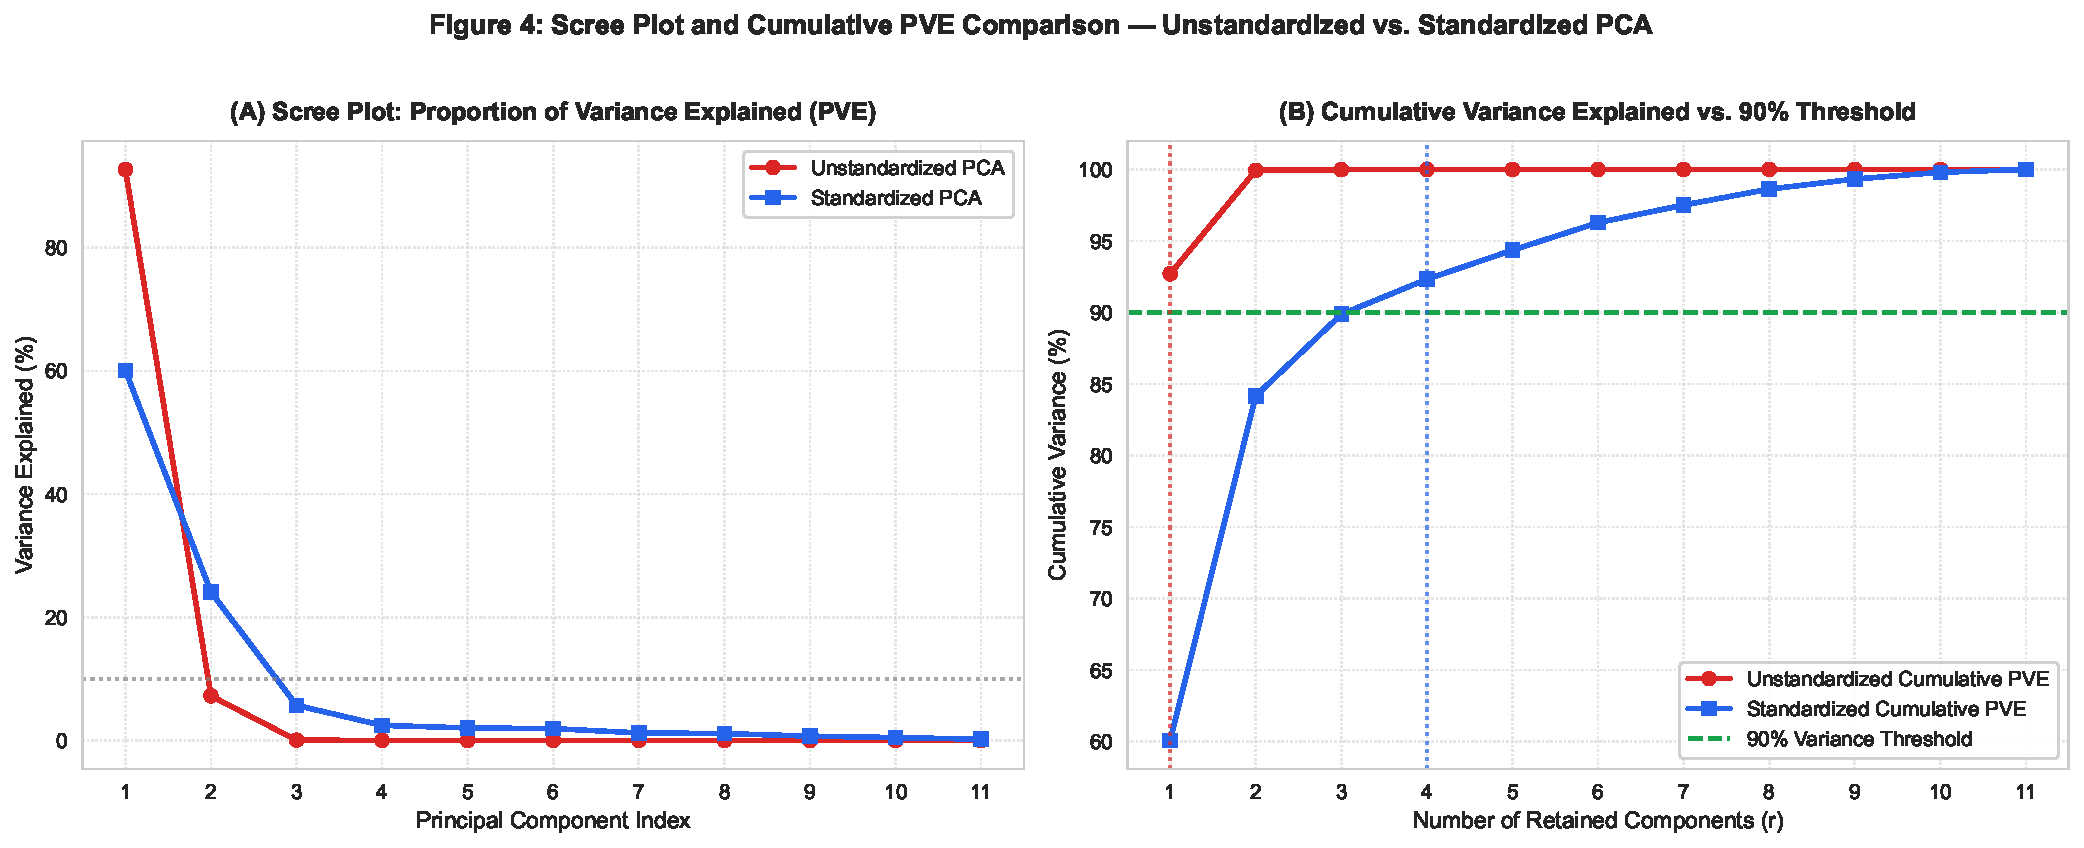
\includegraphics[width=0.96\linewidth]{plot_4_scree_pve_comparison.pdf}
\end{figure}
\vspace{-0.3em}
\begin{tcolorbox}[colback=gray!5!white,colframe=gray!50!black,boxrule=0.5pt,arc=2pt,left=6pt,right=6pt,halign=left,before upper={\sloppy\raggedright},top=4pt,bottom=4pt,unbreakable]
\textbf{Figure 4 — การเปรียบเทียบ Scree Plot และความแปรปรวนสะสม (Cumulative PVE)} Panel (A) กราฟ Scree แสดงสัดส่วนความแปรปรวนที่อธิบายได้ในแต่ละแกน เส้นสีแดง (Unstandardized) ทอดดิ่งลงทันทีเนื่องจาก PC1 แกนเดียวครองไป $92.70\%$ ขณะที่เส้นสีน้ำเงิน (Standardized) กระจายตัวอย่างสมดุล (PC1: $60.08\%$, PC2: $24.10\%$) Panel (B) เส้นความแปรปรวนสะสมเทียบกับเกณฑ์ $90\%$ โดย Unstandardized ถึงเกณฑ์ตั้งแต่ $r=1$ ส่วน Standardized ต้องใช้ $r=4$ ($92.32\%$)
\end{tcolorbox}

\begin{figure}[H]
\centering
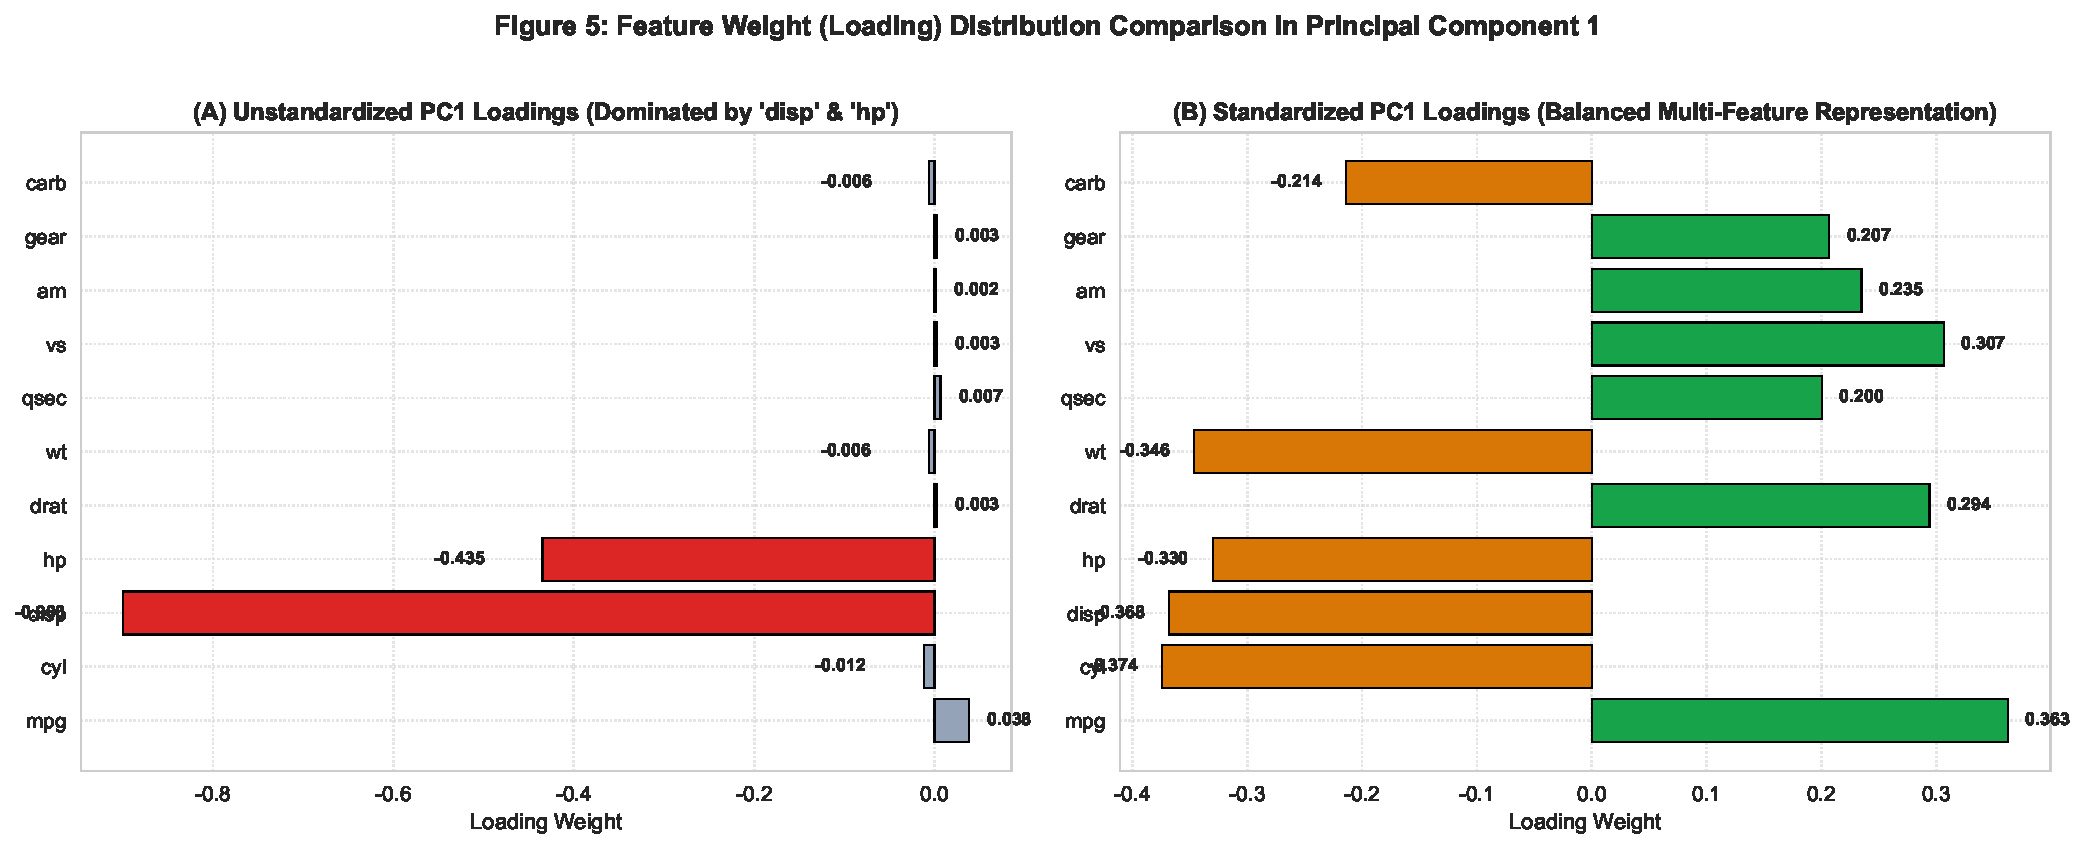
\includegraphics[width=0.96\linewidth]{plot_5_pc_loadings_barplot.pdf}
\end{figure}
\vspace{-0.3em}
\begin{tcolorbox}[colback=gray!5!white,colframe=gray!50!black,boxrule=0.5pt,arc=2pt,left=6pt,right=6pt,halign=left,before upper={\sloppy\raggedright},top=4pt,bottom=4pt,unbreakable]
\textbf{Figure 5 — การแจกแจงค่าน้ำหนัก (Loadings) ของตัวแปรใน PC1} Panel (A) Unstandardized PC1 ถูกครอบงำเกือบสมบูรณ์โดย \texttt{disp} ($-0.900$) และ \texttt{hp} ($-0.435$) ส่วน 9 ตัวแปรที่เหลือมีน้ำหนักใกล้ 0 ทั้งหมด Panel (B) Standardized PC1 มีค่าน้ำหนักกระจายตัวอย่างสมดุลในทุกตัวแปร ($|0.20| - |0.37|$) แบ่งเป็นขั้วกำลังเครื่องยนต์/น้ำหนัก (น้ำหนักลบ) และขั้วประหยัดเชื้อเพลิง/ส่งกำลัง (น้ำหนักบวก)
\end{tcolorbox}

\begin{figure}[H]
\centering
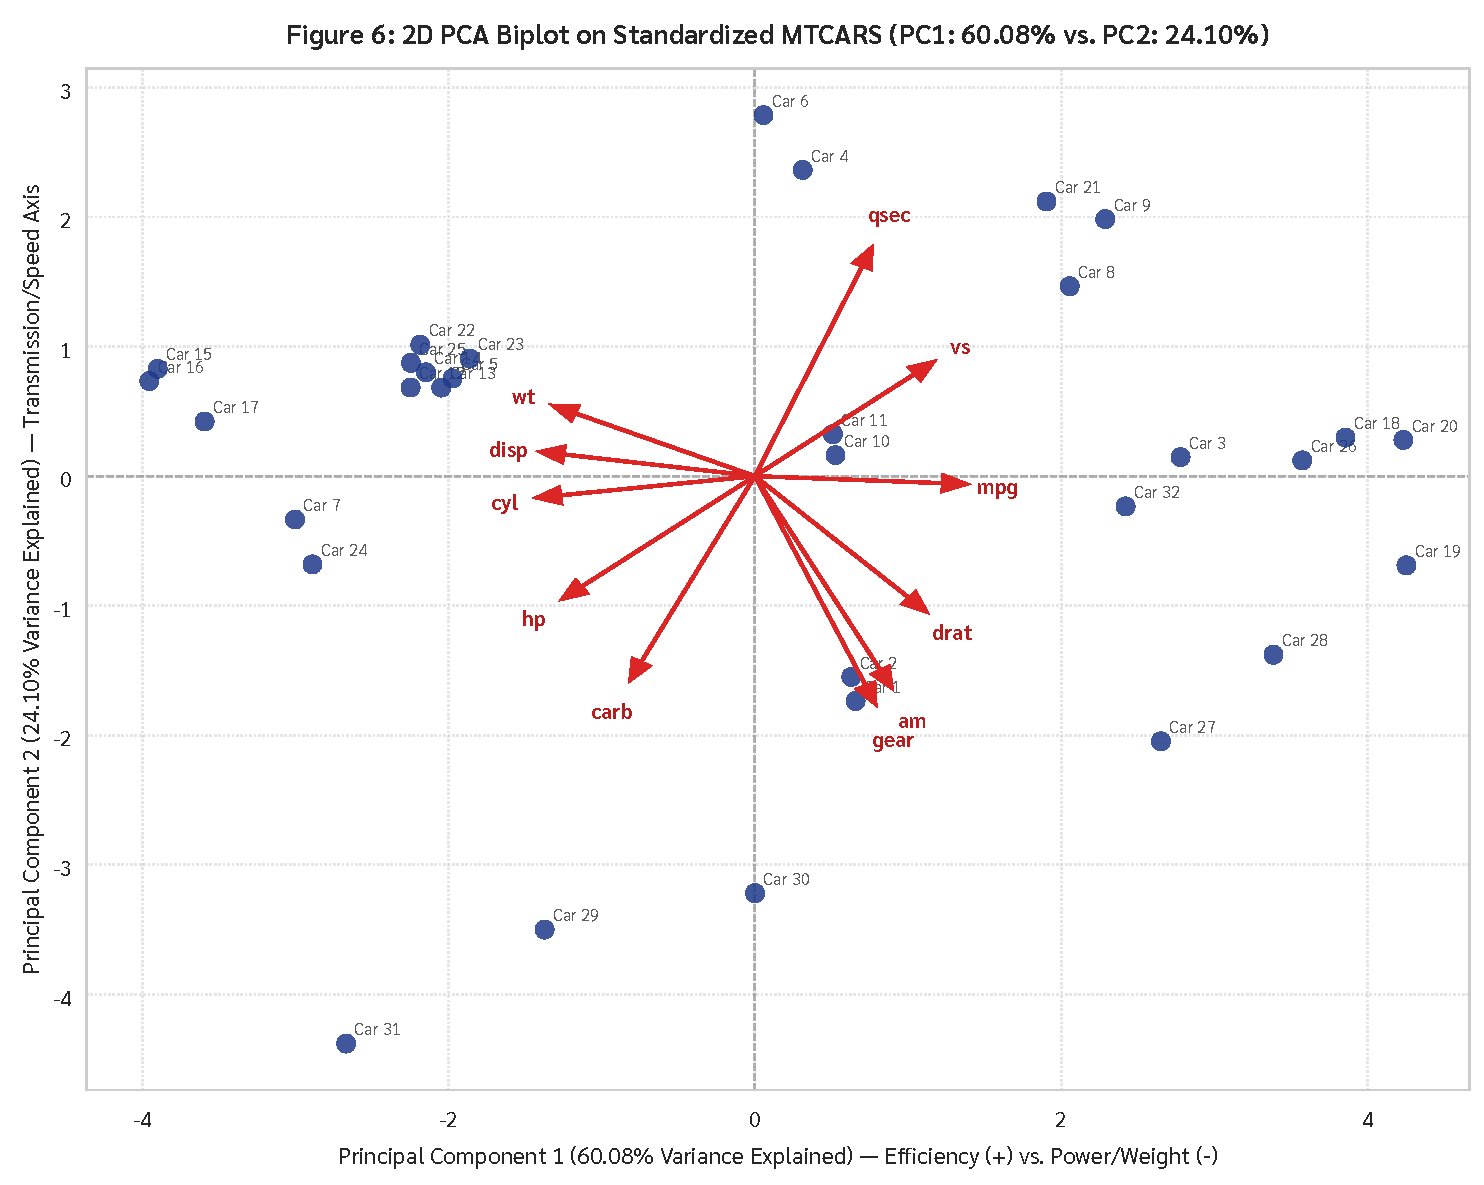
\includegraphics[width=0.96\linewidth]{plot_6_pca_biplot_2d.pdf}
\end{figure}
\vspace{-0.3em}
\begin{tcolorbox}[colback=gray!5!white,colframe=gray!50!black,boxrule=0.5pt,arc=2pt,left=6pt,right=6pt,halign=left,before upper={\sloppy\raggedright},top=4pt,bottom=4pt,unbreakable]
\textbf{Figure 6 — แผนภาพ 2D PCA Biplot บนชุดข้อมูล MTCARS ปรับมาตรฐาน} แสดงการวางตัวของรถยนต์ทั้ง 32 คันบนปริภูมิ PC1 ($60.08\%$) และ PC2 ($24.10\%$) พร้อมเวกเตอร์ลูกศรสีแดงแสดงทิศทางของตัวแปรทั้ง 11 ตัว เวกเตอร์ที่ชี้ไปในทิศทางเดียวกันบ่งบอกสหสัมพันธ์เชิงบวกสูง (เช่น \texttt{cyl}, \texttt{disp}, \texttt{hp}, \texttt{wt}) ซึ่งแยกกลุ่มรถยนต์ Muscle/Luxury รถสปอร์ต และรถประหยัดพลังงานได้อย่างชัดเจน
\end{tcolorbox}

\begin{figure}[H]
\centering
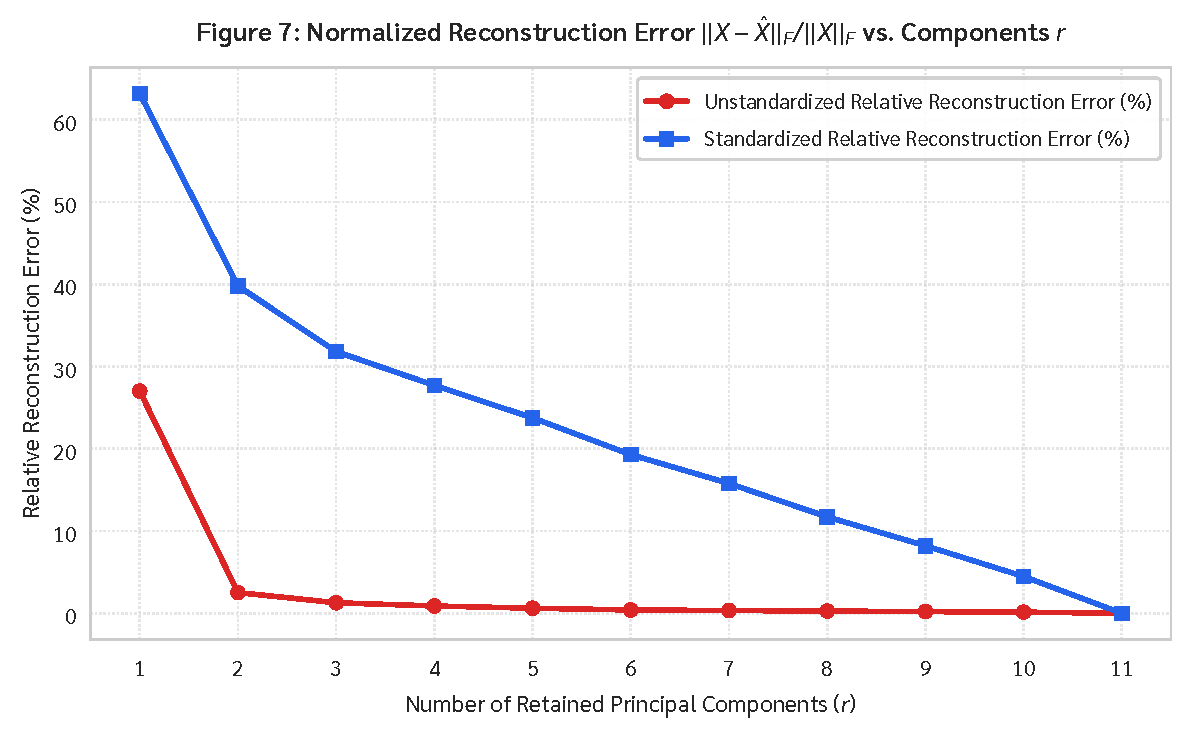
\includegraphics[width=0.96\linewidth]{plot_7_reconstruction_error.pdf}
\end{figure}
\vspace{-0.3em}
\begin{tcolorbox}[colback=gray!5!white,colframe=gray!50!black,boxrule=0.5pt,arc=2pt,left=6pt,right=6pt,halign=left,before upper={\sloppy\raggedright},top=4pt,bottom=4pt,unbreakable]
\textbf{Figure 7 — กราฟข้อผิดพลาดในการฟื้นฟูสัมพัทธ์ (Relative Reconstruction Error) เทียบกับจำนวนองค์ประกอบ $r$} แสดงค่า $\|X - \hat{X}_r\|_F / \|X\|_F \times 100\%$ เมื่อเพิ่มจำนวนมิติ $r$ จาก 1 ถึง 11 ทั้งสองวิธีลดลงสู่ $0\%$ อย่างราบรื่นเมื่อ $r=11$ ยืนยันคุณสมบัติการฟื้นฟูแบบไม่สูญเสียสารสนเทศ (Lossless Reconstruction) ตามทฤษฎี Spectral Theorem
\end{tcolorbox}

\vspace{0.6em}
\needspace{4\baselineskip}
\begin{tcolorbox}[colback=teal!5!white,colframe=teal!60!black,title=\textbf{คำตอบข้อ 2.2 (Question 2.2) — การวิเคราะห์ PCA แบบปรับมาตรฐาน (Standardized PCA)},halign=left,before upper={\sloppy\raggedright},boxrule=0.6pt,arc=3pt,fontupper=\small,top=3pt,bottom=3pt,left=6pt,right=6pt,unbreakable]
\noindent\textbf{\normalsize (a) จำนวน Principal Components (PCs) ที่เพียงพอในการอธิบายความแปรปรวนรวมอย่างน้อย $\approx 90\%$}\par\vspace{0.1em}
\textbf{คำตอบ:} ต้องใช้ \textbf{4 PCs} (เพื่อให้ครอบคลุมเกิน $90\%$ อย่างเคร่งครัด) หรืออนุโลมให้เป็น \textbf{3 PCs} หากยอมรับค่าประมาณใกล้เคียง $90\%$\par
\textbf{หลักฐานเชิงตัวเลข (Cumulative PVE Comparison):}
\begin{itemize}[leftmargin=1.2em, itemsep=0.5pt, topsep=0.5pt]
    \item $\text{PC1}: 60.08\%$
    \item $\text{PC1} + \text{PC2}: 84.17\%$
    \item $\text{PC1} + \text{PC2} + \text{PC3}: 89.87\% \approx 90\%$
    \item $\text{PC1} + \text{PC2} + \text{PC3} + \text{PC4}: \mathbf{92.32\%} > 90\%$
\end{itemize}
\textbf{สรุป:} การปรับมาตรฐานกระจายความแปรปรวนของทุกตัวแปรให้เท่ากันที่ $\sigma^2 = 1.0$ ทำให้ไม่มีตัวแปรใดตัวแปรหนึ่งครองความแปรปรวนเดี่ยว ๆ จึงจำเป็นต้องสะสมถึง \textbf{4 มิติ} เพื่อเก็บข้อมูลให้ครบอย่างน้อย $90\%$\par\vspace{0.2em}

\noindent\textbf{\normalsize (b) ตัวแปรตั้งต้นใดที่ได้ค่าน้ำหนัก (Loadings) สูงใน PC1}\par\vspace{0.1em}
\textbf{คำตอบ:} ใน Standardized PCA \textbf{ตัวแปรทุกตัวมีส่วนร่วมใน $\text{PC1}$ อย่างสมดุล} โดยมีค่าน้ำหนักอยู่ในช่วง $|0.20| - |0.37|$ และแบ่งขั้วการกระจายตัวออกเป็น 2 กลุ่มตรงข้ามอย่างชัดเจน:
\begin{enumerate}[leftmargin=1.2em, itemsep=0.5pt, topsep=0.5pt]
    \item \textbf{กลุ่มค่าน้ำหนักบวก (Efficiency \& Drivetrain Factor):} \texttt{mpg} ($+0.3625$), \texttt{vs} ($+0.3065$), \texttt{drat} ($+0.2942$), \texttt{am} ($+0.2349$), \texttt{gear} ($+0.2069$), \texttt{qsec} ($+0.2005$)
    \item \textbf{กลุ่มค่าน้ำหนักลบ (Power, Displacement \& Weight Factor):} \texttt{cyl} ($-0.3739$), \texttt{disp} ($-0.3682$), \texttt{wt} ($-0.3461$), \texttt{hp} ($-0.3301$), \texttt{carb} ($-0.2140$)
\end{enumerate}
\textbf{การตีความเชิงกายภาพ (Semantic Interpretation):} $\text{PC1}$ ทำหน้าที่เป็นแกน \textbf{``Trade-off ระหว่างขนาด/กำลังเครื่องยนต์ (High Power \& Heavy Weight) กับ ความประหยัดและคล่องตัว (Fuel Efficiency \& Light Mobility)''} ซึ่งสะท้อนโครงสร้างความสัมพันธ์ที่แท้จริงของยานยนต์\par\vspace{0.2em}

\noindent\textbf{\normalsize (c) ผลลัพธ์ของ PCA แตกต่างกันอย่างมีนัยสำคัญหรือไม่ระหว่างการปรับมาตรฐานและไม่ปรับมาตรฐาน? เพราะเหตุใด?}\par\vspace{0.1em}
\textbf{คำตอบ:} \textbf{แตกต่างกันอย่างมหาศาลและมีนัยสำคัญยิ่ง (Dramatically Different)} ดังนี้:
\begin{enumerate}[leftmargin=1.2em, itemsep=0.5pt, topsep=0.5pt]
    \item \textbf{ความหมายของเมทริกซ์ที่นำมาคำนวณ:} Unstandardized PCA ทำบน Sample Covariance Matrix ($\boldsymbol{\Sigma}$) ซึ่งขึ้นกับหน่วยวัด ขณะที่ Standardized PCA ทำบน Pearson Correlation Matrix ($\mathbf{R}$) ซึ่งกำจัดผลของหน่วยวัดออกทั้งหมด (Scale-Invariant)
    \item \textbf{การครอบงำของตัวแปร:} ใน Unstandardized PCA ตัวแปร \texttt{disp} ($\sigma^2 \approx 15,360$) มีขนาดตัวเลขมากกว่าตัวแปรอื่นนับหมื่นเท่า แกน $\text{PC1}$ จึงถูกดึงไปขนานกับแกน \texttt{disp} แทบจะ $100\%$ ขณะที่ Standardized PCA ทุกตัวแปรมี $\text{Var}(z_j) = 1.0$ เท่ากัน จึงมองเห็นสหสัมพันธ์ร่วมได้อย่างแท้จริง
    \item \textbf{ข้อสรุปเชิงปฏิบัติการ (Engineering Recommendation):} เมื่อชุดข้อมูลประกอบด้วยตัวแปรที่มีหน่วยวัดต่างกัน \textbf{จำเป็นอย่างยิ่งที่จะต้องทำ Data Standardization ก่อนประยุกต์ใช้ PCA เสมอ}
\end{enumerate}
\end{tcolorbox}



\end{document}
